\documentclass[a5paper,9pt,fleqn,twoside]{scrartcl}

% packages
\usepackage[ngerman]{babel}
\usepackage[german]{fancyref}
\usepackage{amsmath, amssymb}
\usepackage[locale=DE]{siunitx}
\usepackage{mdwlist}
\usepackage{array}
%\usepackage{scrpage2}
\usepackage{booktabs}
\usepackage{multirow}
\usepackage{multicol}
\usepackage{tikz}
\usepackage{pgfplots}
\usepackage{footnote}
\usepackage{caption}
\usepackage{tabularx} 
\usepackage{float}
\usepackage{rotating}
\usepackage{xcolor}
\usepackage{environ}
%\usepackage{microtype}
\usepackage{enumitem}
\usepackage{geometry}
\usepackage{fancyhdr}
\usepackage{prettyref}



% setup
\providecommand{\abs}[1]{\left| #1 \right|}
\providecommand{\ergebnis}[1]{\begin{center}\framebox{#1}\end{center}}
\providecommand{\errorterm}[2]{\ensuremath{\abs{\frac{\partial #2}{\partial #1}}\Delta #1}}
\providecommand{\grad}[1]{\ensuremath{\text{grad}\;#1}}
\providecommand{\degree}[0]{\ensuremath{\,^\circ}}
\providecommand{\ohm}[0]{\ensuremath{\Omega}}
\renewcommand{\epsilon}[0]{\varepsilon}


\newenvironment{eeqn}[1]%
% BEGIN 
{%
	\begin{minipage}{\textwidth}%
	\begin{minipage}{0.35\linewidth}%
		\begin{flushleft}\textbf{\sffamily #1}\end{flushleft}%
	\end{minipage}%
	\hspace{0.02\linewidth}%
	\begin{minipage}{0.63\linewidth}%
}%
% END
{%
	\end{minipage}%
	\\[8pt]%
	\hrule%
	\end{minipage}\\%
}


\NewEnviron{vardef}{
	\colorbox{gray!30}{%
	\begin{minipage}{0.98\linewidth}%
	\textbf{\sffamily Nomenklatur}		
	\begin{multicols}{2}%
	\begin{description*}%
		\BODY
	\end{description*}%
	\end{multicols}%
	\end{minipage}%
	}%
	\vspace{10pt}
}

\sisetup{separate-uncertainty=true}
\usetikzlibrary{arrows}
\usetikzlibrary{decorations} 
\pgfplotsset{compat=1.3}

% layout
\usepackage[T1]{fontenc}
\usepackage[utf8]{inputenc}
\usepackage[final]{pdfpages}
\parindent0pt
\geometry{a5paper, twoside, left=20mm,right=10mm, top=15mm, bottom=20mm}
\setlength{\mathindent}{0mm}
\setlength{\columnseprule}{.4pt}

% meta data 
\title{Römerturm Version 1.3.1}
\subject{Formelsammlung Konstruktionselemente}

\author{Stefan Bürgel \and Andreas Jendrzey \and Christoph Hansen \\ 
Emailkontakt: uni@christophhansen.eu}

\date{}

% kopf und fußzeile
\renewcommand{\headrulewidth}{0.8pt}
\pagestyle{fancy}
\fancyfoot{}
\fancyhead[LE,RO]{\thepage}
\fancyhead[RE,LO]{\leftmark}


\begin{document}
% Cover
\thispagestyle{empty}
\cleardoublepage
% Titelseite / Inhaltsverzeichnis
\maketitle


\textcolor{red}{Ich erhebe keinen Anspruch auf Vollständigkeit oder Richtigkeit. Falls ihr Fehler findet oder etwas fehlt, dann meldet euch bitte über den Emailkontakt.}

\setcounter{page}{1}
\begin{multicols}{2}
	\tableofcontents
\end{multicols}
	\pagebreak
	\section{Festigkeitslehre}
\subsection{Spannungen}
% E => G
\hrule
\begin{eeqn}{Umrechnung zwischen Schubmodul $G$ und Elastizitätsmodul $E$}
 		\begin{flalign}
 			G &= \frac{E}{2(1+\mu)}
		\end{flalign}
		Für Stähle gilt $\mu=0,33$
\end{eeqn}
\begin{figure}[H]
	\begin{minipage}[b]{0.22\linewidth}
		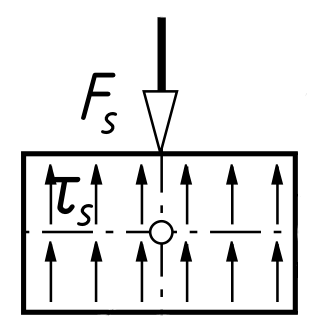
\includegraphics[width=\linewidth]{festigkeitslehre/scherung}
		\caption*{Scherspannungen}
	\end{minipage}
	\begin{minipage}[b]{0.5\linewidth}
		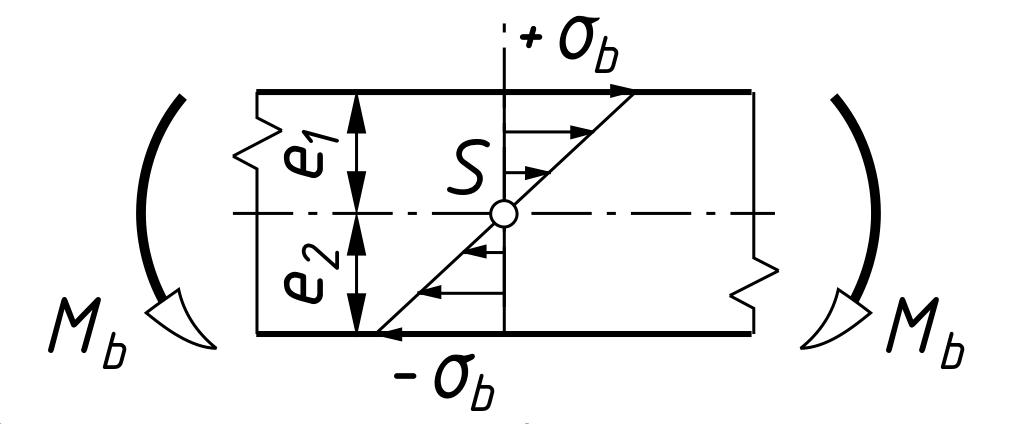
\includegraphics[width=\linewidth]{festigkeitslehre/biegung}
		\caption*{Biegespannungen}
	\end{minipage}
	\begin{minipage}[b]{0.26\linewidth}
		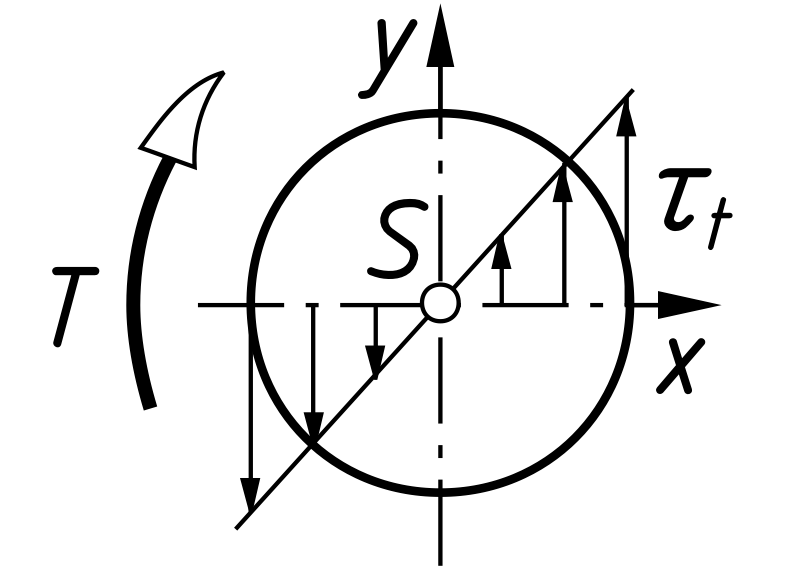
\includegraphics[width=\linewidth]{festigkeitslehre/torsion}
		\caption*{Torsionsspannungen}
	\end{minipage}
\end{figure}
% Biegespannungen
\hrule
\begin{eeqn}{Biegespannungen}
 		\begin{flalign}
 			\sigma_\text{B} & = \frac{M_\text{B}}{W_\text{ax}}
		\end{flalign}
\end{eeqn}
% Torsionsspannungen
\begin{eeqn}{Torsionsspannungen}
 		\begin{flalign}
 			\tau_\text{t} & = \frac{M_\text{t}}{W_\text{t}}
		\end{flalign}
		Für Kreis- und Rohrgeometrien ist $W_\text{t}=W_\text{p}$
\end{eeqn}
% Scherspannungen
\begin{eeqn}{Scherspannungen}
 		\begin{flalign}
 			\tau_\text{A} & = \frac{F_\text{A}}{A}
		\end{flalign}
\end{eeqn}

\subsection{Widerstandsmomente}
\begin{table}[H]
\begin{tabularx}{\linewidth}{m{30mm}XX}
	\toprule
	Geometrie & $I$ & $W$ \\
	\midrule
	% Kreis
	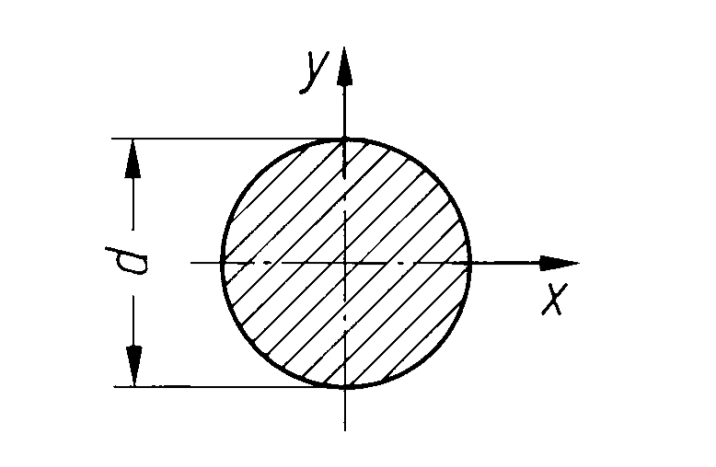
\includegraphics[width=30mm]{festigkeitslehre/kreis} & $\begin{aligned} & I_\text{ax} = \frac{\pi d^4}{64} \\ &I_\text{p} = \frac{\pi d^4}{32}\end{aligned}$ & $\begin{aligned} &W_\text{ax} = \frac{\pi d^3}{32} \\ &W_\text{p}=\frac{\pi d^3}{16}\end{aligned}$\\ \midrule
	% Kreisring
	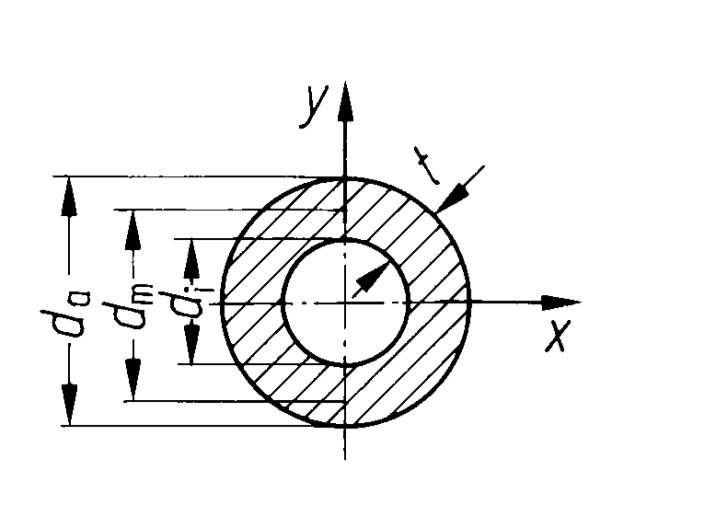
\includegraphics[width=30mm]{festigkeitslehre/kreisring} & $\begin{aligned} & I_\text{ax} = \frac{\pi (d_\text{a}^4-d_\text{i}^4)}{64} \\ &I_\text{p} = \frac{\pi (d_\text{a}^4-d_\text{i}^4)}{32}\end{aligned}$ & $\begin{aligned}& W_\text{ax} = \frac{\pi (d_\text{a}^4-d_\text{i}^4)}{32\cdot d_\text{a}} \\ &W_\text{p}=\frac{\pi (d_\text{a}^4-d_\text{i}^4)}{16\cdot d_\text{a}} \end{aligned}$\\ \midrule
	% Rechteck
	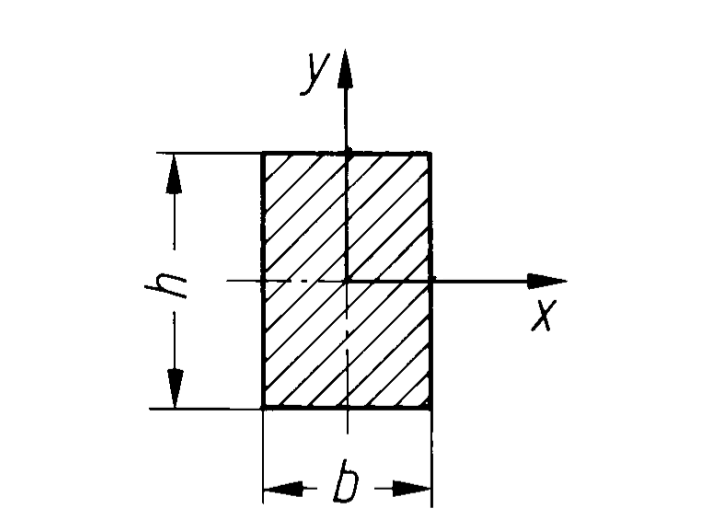
\includegraphics[width=30mm]{festigkeitslehre/rechteck} & $\begin{aligned} & I_\text{x} = \frac{bh^3}{12} \\ &I_\text{y} = \frac{b^3h}{12} \end{aligned}$ & $\begin{aligned} W_\text{x} = \frac{bh^2}{6} \\ W_\text{y} = \frac{b^2h}{6}\end{aligned}$ \\ \midrule
	% Quadrat
	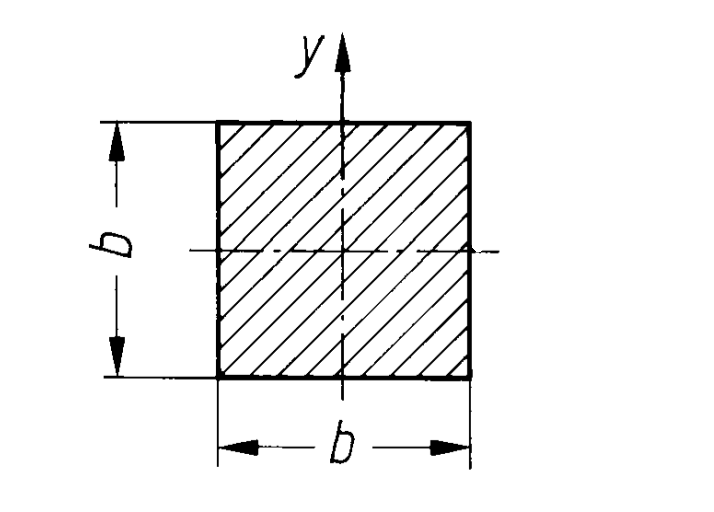
\includegraphics[width=30mm]{festigkeitslehre/quadrat} & $\begin{aligned} & I_\text{ax} = \frac{b^4}{12} \end{aligned}$ & $\begin{aligned} W_\text{ax} = \frac{b^3}{6} \end{aligned}$ \\ \midrule
	% Dreieck
	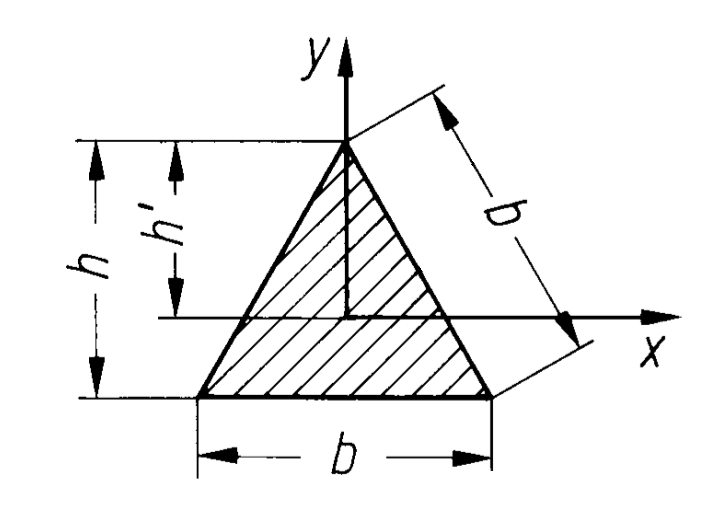
\includegraphics[width=30mm]{festigkeitslehre/dreieck} & $\begin{aligned} & I_\text{x} = \frac{bh^3}{36} \\ &I_\text{y} = \frac{b^3h}{48} \end{aligned}$ & $\begin{aligned} W_\text{x} = \frac{bh^2}{24} \\ W_\text{y} = \frac{b^2h}{24}\end{aligned}$ \\\bottomrule
\end{tabularx}
\end{table}
\vfill
\pagebreak

\subsection{Mohr'scher Spannungskreis}
\begin{figure}[H]
	\centering
	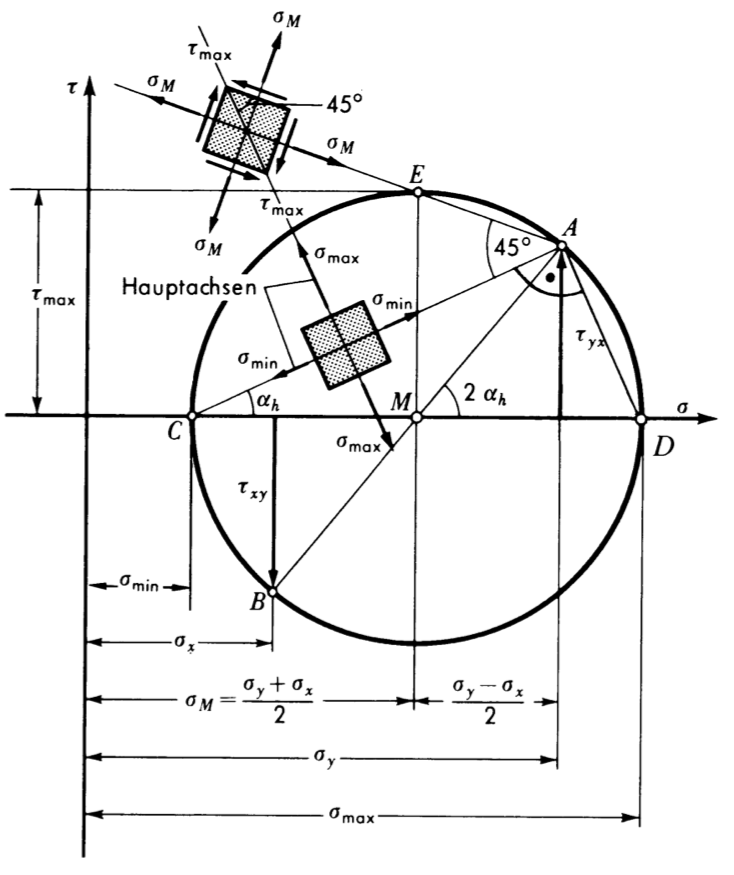
\includegraphics[width=0.63\linewidth]{festigkeitslehre/mohrischer-spannungskreis}
	\caption*{Mohrischer Spannungskreis}
\end{figure}

% maximale Spannungen
\hrule
\begin{eeqn}{max/min Spannnungen}
	\begin{flalign}
		\sigma_{1,2} & = \frac{\sigma_\text{x}+\sigma_\text{y}}{2} \pm \frac{1}{2} \sqrt{(\sigma_\text{x}-\sigma_\text{y})^2+4\tau_\text{xy}^2} 
	\end{flalign}
	Im Mohr'schem Spannungskreis befinden sich diese Spannungen bei den Nullstellen auf der Spannungsachse, auch Hauptspannungen genannt.
\end{eeqn}

% Winkel
\begin{eeqn}{gedrehte Spannungen}
	\begin{flalign}
		\tan 2\alpha & = \frac{2\tau_\text{xy}}{\sigma_\text{x}-\sigma_\text{y}}
	\end{flalign}
	Der Winkel $\alpha$ gibt an, um wie viel Grad das Koordinatensystem gedreht wird. Setzt man $\tau_\text{xy} = 0$, erhält man den Winkel unter dem die Hauptspannungen auftreten. 
\end{eeqn}

\subsection{Vergleichs\-spannungs\-hypothesen}
% NSH
\hrule
\begin{eeqn}{Normalspannungs\-hypothese (NSH)}
	\begin{flalign}
		\sigma_\text{v} & = \frac{\abs{\sigma_\text{x}+\sigma_\text{y}}}{2} + \frac{1}{2} \sqrt{(\sigma_\text{x}-\sigma_\text{y})^2+4\tau_\text{xy}^2}
	\end{flalign}
	Die Vergleichsspannung $\sigma_\text{v}$ entspricht der maximalen Normalspannung.
\end{eeqn}

% SSH
\begin{eeqn}{Schubspannungs\-hypothese (SSH)}
	\begin{align}
		&\sigma_1 > \sigma_2 > 0: &\quad \sigma_\text{v} &= \sigma_1 \\
		& \sigma_1 > 0 > \sigma_2: &\quad  \sigma_\text{v}& = \sigma_1 - \sigma_2 \\
		& 0 > \sigma_1 > \sigma_2: &\quad \sigma_\text{v} &= \abs{\sigma_2}
	\end{align}
	Die Vergleichsspannung $\sigma_\text{v}$ entspricht der maximalen Schubspannung.
\end{eeqn}

% GEH
\begin{eeqn}{Gestaltänderungs\-hypothese (GEH)}
	\begin{flalign}
		\sigma_\text{v} &= \sqrt{\sigma_{x}^2+\sigma_{y}^2-\sigma_{x}\sigma_{y}+3\tau_\text{xy}^2}
	\end{flalign}
	Diese Formel entspricht einem zweiachsigen Spannungszustand. Für mehrachsige Spannungszustände siehe Skript. I.d.R: $\tau_\text{xy}^2 = \tau_\text{A}^2+ \tau_\text{t}^2$
\end{eeqn}
\vfill
\pagebreak


\subsection{Dauerfestigkeit}
\begin{vardef}
	\item[$\beta_\text{k}$] Kerbwirkungsfaktor
	\item[$b_1$] Oberflächenbeiwert (siehe Diagramm: ad gegen $R_\text{m}$)
	\item[$b_2$] Größenbeiwert (siehe Diagramm: Wellendruchmesser)
	\item[$\sigma_\text{z, sch}$] Maximal auftretende Spannungen bei reiner Zugschwellbelastung
	\item[$\sigma_\text{gak}$] Ausschlagsspannung unter Berücksichtigung von Gestalt und Kerbwirkung
	\item[$\sigma_\text{gk,zdw}$] Zug- Druck Wechselspannung unter Berücksichtigung von Gestalt und Kerbwirkung 
\end{vardef}

\begin{figure}[H]
	\centering
	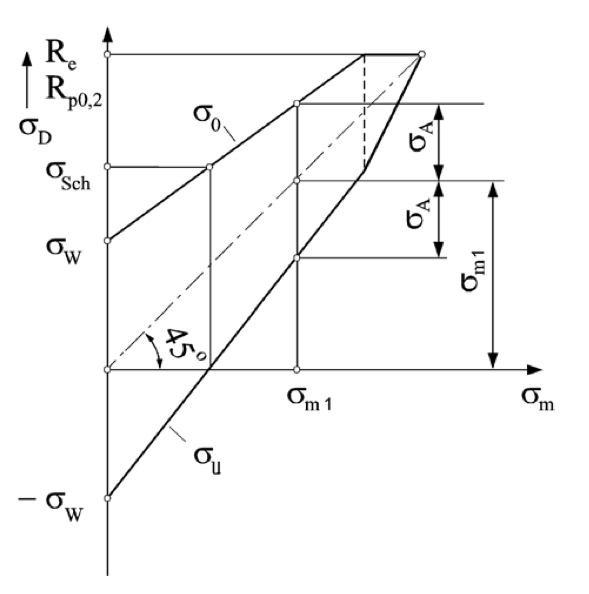
\includegraphics[width=0.5\linewidth]{festigkeitslehre/smith-diagramm}
	\caption*{Dauerfestigkeitsdiagramm nach Smith}
\end{figure}

\hrule
% 1. Reduktion
\begin{eeqn}{1. Reduktion}
	\begin{flalign}
		& \sigma_\text{z, zul}^* = R_\text{e} \cdot b_2 \\
		& \sigma_\text{zdw}^* = \sigma_\text{zdw} \cdot b_2\\
		& \sigma_\text{z, sch}^* = \sigma_\text{z, sch} \cdot b_2 \\
		& \sigma_\text{a}^* = \sigma_\text{a} \cdot b_2
	\end{flalign}
\end{eeqn}
\begin{eeqn}{2. Reduktion}
	\begin{flalign}
		& K = \frac{b_1}{\beta_\text{k}}\\
		& \sigma_\text{gak} = \sigma_\text{a}^*\cdot K \\
		& \sigma_\text{gzdw} = \sigma_\text{zdw}^* \cdot K
	\end{flalign}
\end{eeqn}

	\section{Achsen und Wellen}
\subsection{Auslegung von Achsen}
\hrule
% erforderlicher Durchmesser
\begin{eeqn}{erforderlicher Durchmesser}
	\begin{flalign}
		d_\text{erf} & = \sqrt[3]{\frac{32\cdot M_\text{B, max}}{\pi \cdot \sigma_\text{B,zul}}}
	\end{flalign}
	Wenn sich der erforderliche Durchmesser dynamisch zum momentanen Biegemoment bestimmt werden soll, ergibt sich für $d_\text{erf} = d_\text{erf}(x)$ und $M_\text{B}=M_\text{B}(x)$.
\end{eeqn}

\subsection{Auslegung von Wellen}
\begin{vardef}
	\item[$P$] Leistung, die die Welle überträgt.
	\item[$\omega$] Winkelgeschwindigkeit.
	\item[$n$] Drehzahl in $\text{min}^{-1}$
	\item[$M_\text{v}$] Vergleichsmoment
\end{vardef}
\hrule
% Drehzahl
\begin{eeqn}{Drehzahl}
	\begin{flalign}
		\omega & = \frac{2\pi\cdot n}{60}
	\end{flalign}
\end{eeqn}

% Drehmoment
\begin{eeqn}{Drehmoment}
	\begin{flalign}
		M &= \frac{P}{\omega}
	\end{flalign}
\end{eeqn}

% Vergleichsmoment / erforderlicher Durchmesser
\begin{eeqn}{erforderlicher Durchmesser}
	\begin{flalign}
		& M_\text{v} = \sqrt{M_\text{B}^2+\frac{3}{4}\cdot M_\text{t}^2}\\
		& d_\text{erf} = \sqrt[3]{\frac{32\cdot M_\text{v}}{\sigma_\text{zul} \cdot \pi}}
	\end{flalign}
	Die Wirkung von Torsion $M_\text{t}$ und Biegung $M_\text{B}$ werden im Vergleichsmoment $M_\text{v}$ kombiniert. 
\end{eeqn}
	\section{Federn}
\subsection{Grundlagen}

\hrule
% Hook'sches Gesetz
\begin{eeqn}{Hook'sches Gesetz}
	\begin{align}
		&\text{Normalfedern:}  &\quad  F &= c\cdot x & [c] &=\text{N/mm}\\
		&\text{Torsionsfedern:}&\quad  M &= c\cdot \alpha & [c] &=\text{Nmm}
	\end{align}
\end{eeqn}

% Federarbeit
\begin{eeqn}{Federarbeit}
	\begin{align}
		&\text{Normalfedern:}  &\quad W = \frac{1}{2} \cdot c \cdot x^2 \\
		&\text{Torsionsfedern:}&\quad  W = \frac{1}{2} \cdot c \cdot \alpha^2
	\end{align}
\end{eeqn}

% Zusammengeschaltete Federn: Reihenschaltung
\begin{eeqn}{Reihenschaltung}
	\begin{align}
		\frac{1}{c_\text{ges}} = \frac{1}{c_1} + \frac{1}{c_2} + \dots + \frac{1}{c_\text{n}}
	\end{align}
	Für die Reihenanordnung von Federn gilt die Bedingung, dass auf alle beteiligten Federn die selbe Kraft wirkt. ($F_1 = F_2 = \dots = F_\text{n}$)
\end{eeqn}

% Zusammengeschaltete Federn: Parallelschaltung
\begin{eeqn}{Parallelschaltung}
	\begin{align}
		c_\text{ges} = c_1 + c_2 + \dots + c_\text{n}
	\end{align}
	Für die Reihenanordnung von Federn gilt die Bedingung, dass alle beteiligten Federn den selben Weg zurücklegen. ($s_1 = s_2 = \dots = s_\text{n}$)
\end{eeqn}

\begin{figure}[H]
	\centering
	\begin{minipage}[b]{0.30\linewidth}
		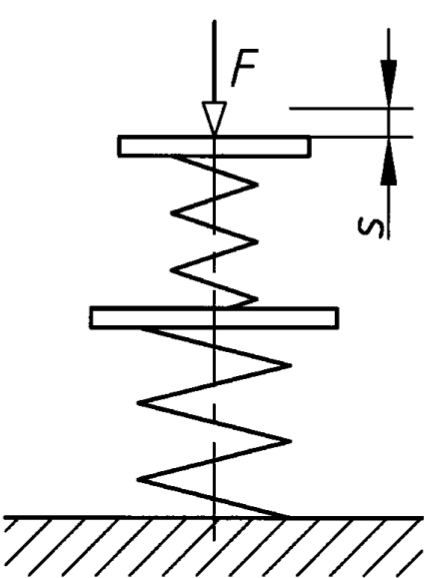
\includegraphics[width=\linewidth]{federn/reihenschaltung}
		\vspace{3.6mm}
		\caption*{Reihenschaltung}
	\end{minipage}
	\begin{minipage}[b]{0.43\linewidth}
		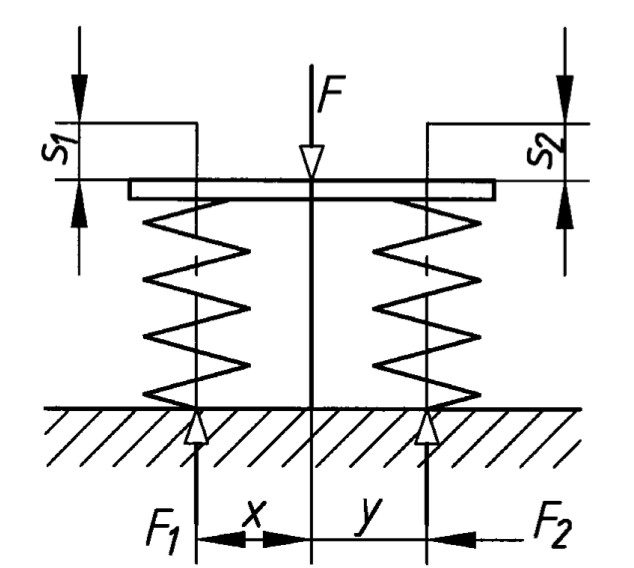
\includegraphics[width=\linewidth]{federn/parallelschaltung}
		\caption*{Parallelschaltung}
	\end{minipage}
\end{figure}


\pagebreak

\subsection{Blattfedern}
\begin{vardef}
	\item[$b$] maximale Breite der Feder.
	\item[$b'$] minimale Breite der Feder.
	\item[$b_0$] Breite der geschichteten Blattfeder.
	\item[$z$] Gesamtzahl der Blätter.
	\item[$z'$] Anzahl der Blätter mit der Gesamtlänge $L$.
	\item[$s$] Dicke der Feder.
	\item[$q_1$] Korrekturfaktor zur Berücksichtigung der Bauform
	\item[$f$] Federweg
\end{vardef}

\begin{tabularx}{\textwidth}{m{15mm}m{17mm}m{20mm}m{20mm}XX}
    \toprule
		Typ & $b(x)$ & $W_\text{ax}(x)$ & $\sigma_\text{B}(x)$ & $\sigma_\text{B,max}$ & $q_1$ \\ \midrule
		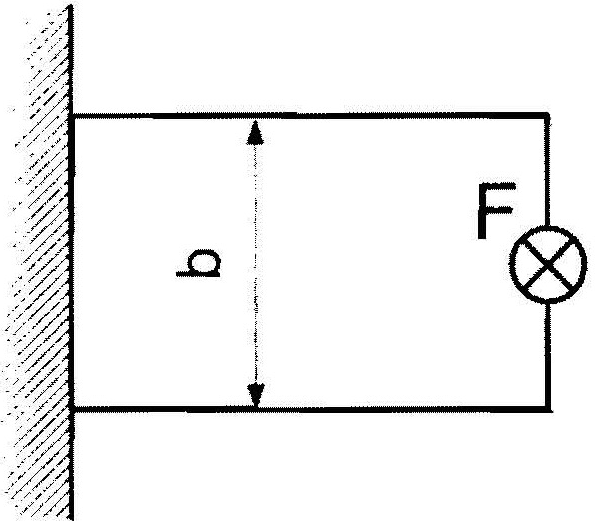
\includegraphics[width=15mm]{federn/blattfedern-rechteck} & const. & $\frac{b\cdot s^2}{6}$ & $\frac{6\cdot F \cdot x}{b\cdot s^2}$ & $\frac{6\cdot F \cdot L}{b \cdot s^2}$ & 4\\
		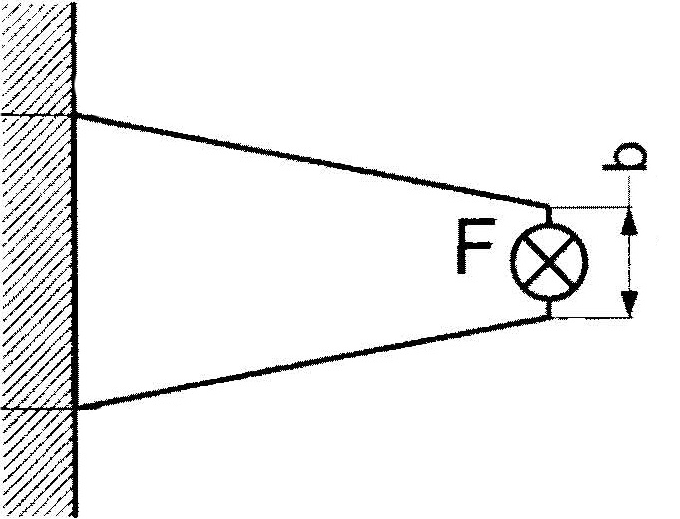
\includegraphics[width=15mm]{federn/blattfedern-trapez} & $b'+\frac{x \cdot (b-b')}{L}$ & $\frac{s^2\cdot [b'+\frac{x}{L}(b-b')]}{6}$ & $\frac{6\cdot F \cdot x}{s^2[b'+\frac{x}{L}(b-b')]}$ & $\frac{6\cdot F \cdot L}{b \cdot s^2}$ & $\frac{12}{2+b'/b}$\\
		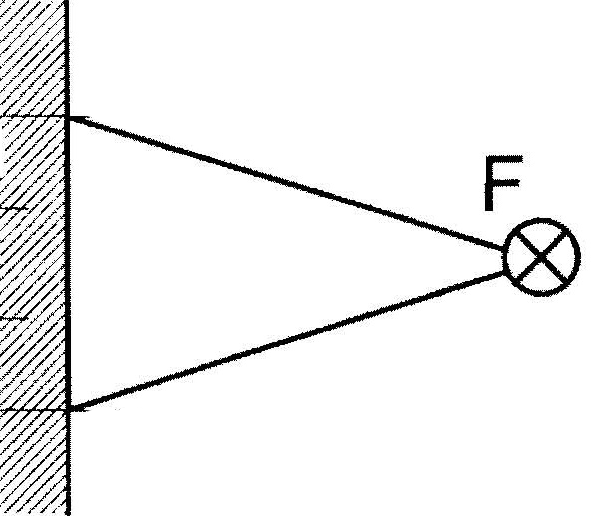
\includegraphics[width=15mm]{federn/blattfedern-dreieck} & $\frac{x \cdot b}{L}$ & $\frac{b\cdot s^2 \cdot x}{6\cdot L}$ & $\frac{6\cdot F \cdot L}{b\cdot s^2}$ & $\frac{6\cdot F \cdot L}{b \cdot s^2}$ & 6\\
    \bottomrule
\end{tabularx}
\\[10pt]
\hrule
% Federrate
\begin{eeqn}{Federrate}
	\begin{align}
		c &= \frac{b\cdot s^3 \cdot E}{q_1 \cdot L^3}
	\end{align}
	Die Federrate ist eine Funktion der Geometrie ($q_1$, $b$ und $s$) und des Werkstoffs $E$.
\end{eeqn}

% Federweg
\begin{eeqn}{Federweg}
	\begin{align}
		f &= q_1 \cdot \frac{L^3}{b\cdot s^3}\cdot \frac{F}{E}
	\end{align}
\end{eeqn}

% max. Federweg
\begin{eeqn}{maximaler Federweg}
	\begin{align}
		f_\text{max} &= q_1 \cdot \sigma_\text{B,zul} \cdot \frac{L^2}{6 \cdot s \cdot E}
	\end{align}
\end{eeqn}

\begin{figure}[H]
	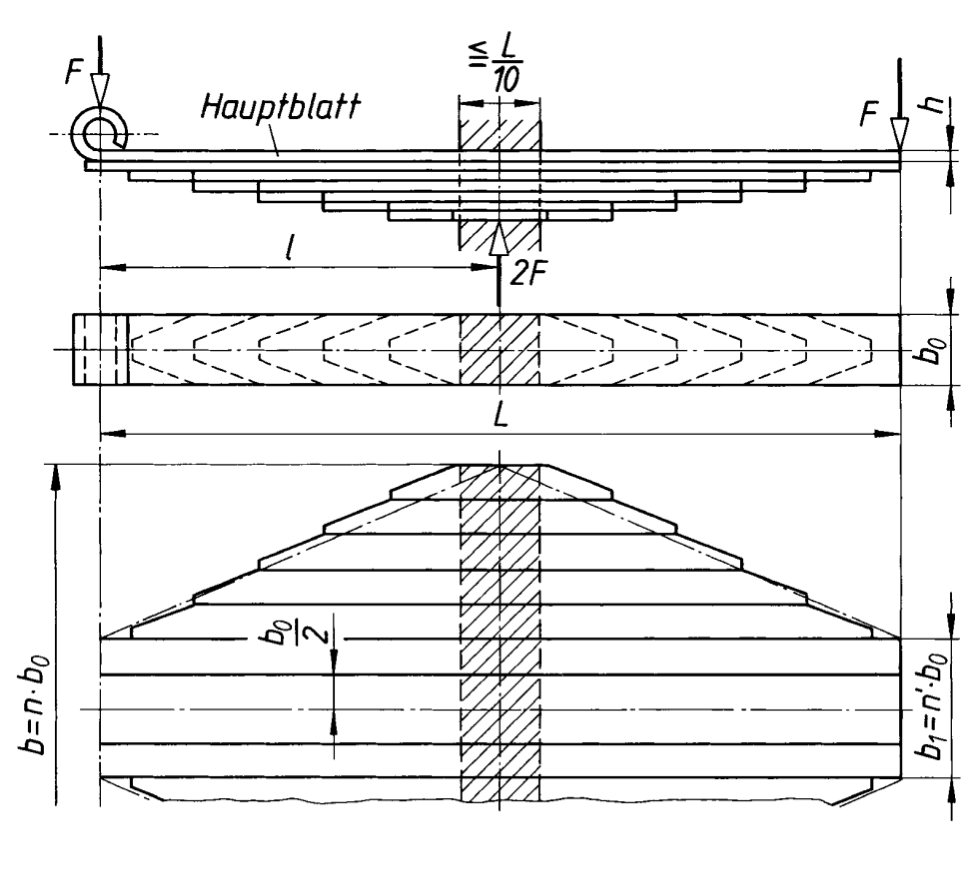
\includegraphics[width=\linewidth]{federn/blattfedern-geschichtet}
	\caption*{Geschichtete Blattfedern}
\end{figure}

% geschichtete Blattfedern
\hrule
\begin{eeqn}{geschichtete Blattfedern}
	Geschichtete Blattfedern verhalten sich wie Trapezfedern mit folgenden Einschränkungen:
	\begin{align}
		&q_1  = \frac{12}{2+\frac{z'}{z}}\\
		&b' = z'\cdot b_0 \\
		&b  = z \cdot b_0
	\end{align}
\end{eeqn}

\subsection{Drehfedern (Biegefedern)}
\begin{vardef}
	\item[$L$] Länge der abgewickelten Feder (Drahtlänge)
	\item[$L^*$] Länge einer Windung
	\item[$i_\text{F}$] Anzahl der Windungen
	\item[$\alpha_0$] Winkel der Federenden zueinander.
	\item[$a$] Abstand der unbelasteten Windungen (in Rad)
	\item[$d$] Drahtdurchmesser
	\item[$D_\text{a}$] Außendurchmesser der Feder
	\item[$D_\text{i}$] Innendurchmesser der Feder
	\item[$D_\text{m}$] Mittlerer  Durchmesser der Feder
	\item[$L_\text{K}$] Gesamtlänge des Federkörpers
\end{vardef}
\begin{figure}[H]
	\centering
	\begin{minipage}[b]{0.45\linewidth}
		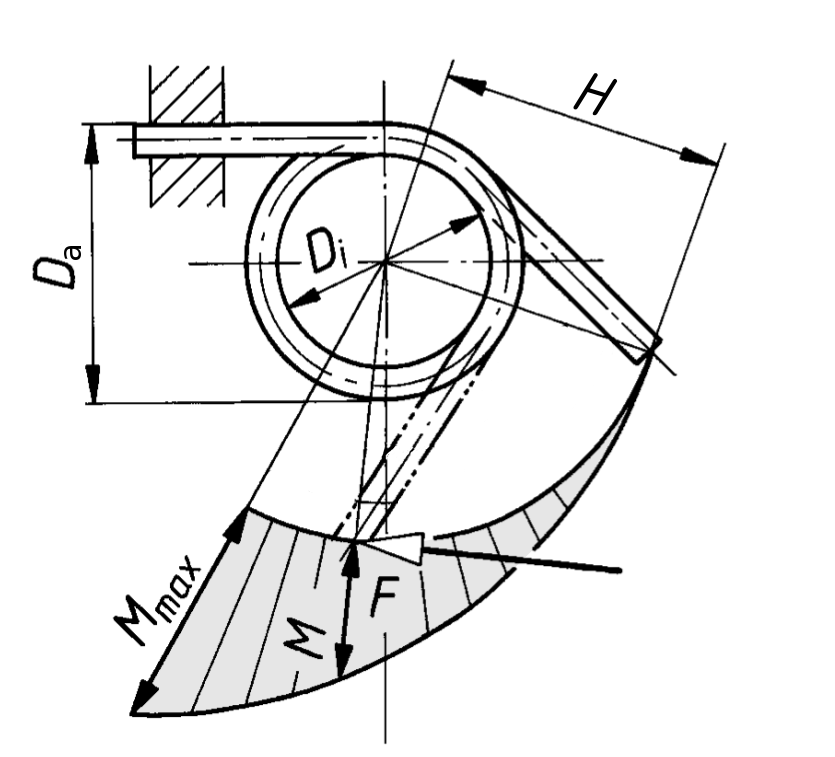
\includegraphics[width=\linewidth]{federn/drehfedern}
		\caption*{Belastung einer Drehfeder}
	\end{minipage}
	\begin{minipage}[b]{0.45\linewidth}
		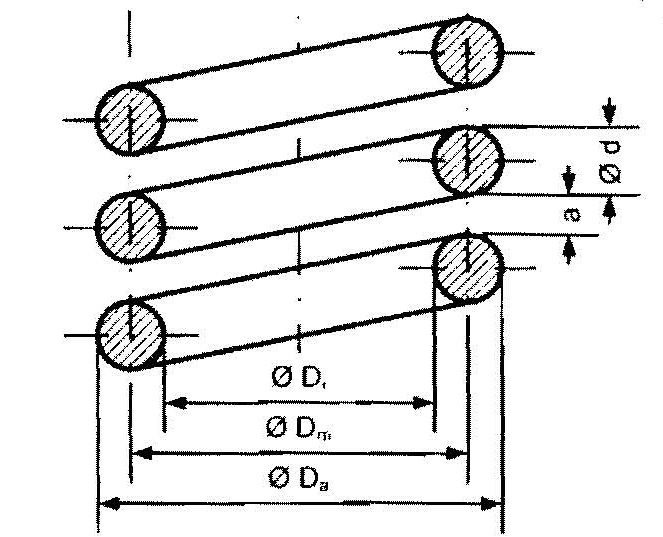
\includegraphics[width=\linewidth]{federn/drehfedern-geometrie}
		\caption*{Geometrie einer Drehfeder}
	\end{minipage}
\end{figure}

\hrule
% Wicklungsverhältnis
\begin{eeqn}{Wicklungsverhältnis}
	\begin{align}
		W &= \frac{D_m}{d}
	\end{align}
\end{eeqn}

% Federgeometrie
\begin{eeqn}{Federgeometrie}
	\label{sec:federgeometrie-drehfedern}
	\begin{align}
		& D_\text{a} = D_\text{m} + d \\
		& D_\text{i} = D_\text{m} - d \\
		& L = i_\text{F} \cdot L^*
	\end{align}
\end{eeqn}

% Länge einer Windung
\begin{eeqn}{Länge einer Windung}
	Wenn $(a+d) \leq 0,25\cdot D_\text{m}$, dann gilt:
	\begin{align}
         L^* &= \pi \cdot D_\text{m}
    \end{align}
    anderenfalls gilt:
    \begin{align}
    	L^* = \sqrt{(D_\text{m}\cdot\pi)^2+(a+d)^2}
    \end{align}
\end{eeqn}

% Korrekturfaktor durch Spannnungserhöhungen an der Innenseite
\begin{eeqn}{Korrekturfaktor durch Spannnungserhöhungen an der Innenseite}
	\begin{align}
		q & = \frac{W+0,07}{W-0,75}
	\end{align}
	Beim Auslegen von Federn wird $q=1$ gesetzt, später wird dann der tatsächliche Wert von $q$ bestimmt.
\end{eeqn}

% Spannungen in der Feder
\begin{eeqn}{Spannungen in der Feder}
	\begin{align}
		\sigma_\text{B} & = \frac{F\cdot H \cdot 32}{\pi \cdot d^3} \cdot q
	\end{align}
	Hierbei entspricht $H$ dem Hebelarm, welcher die Kraft $F$ zum Mittelpunkt der Feder aufweist. Alternativ kann auch $M = F\cdot H$ gesetz werden.
\end{eeqn}

% Federrate
\begin{eeqn}{Federrate}
	\begin{align}
		c & = \frac{I_\text{ax}\cdot E}{L} = \frac{M}{\alpha}
	\end{align}
\end{eeqn}

% Winkel der Federenden
\begin{eeqn}{Winkel der Federenden zueinander}
		Die Nachkommerstellen von $i_\text{F}$ geben an, in welchem Winkel die Enden der Feder zueinander stehen. Diesen Winkel nennt man auch gewickelten Grundwinkel.
		\begin{figure}[H]
			\centering
			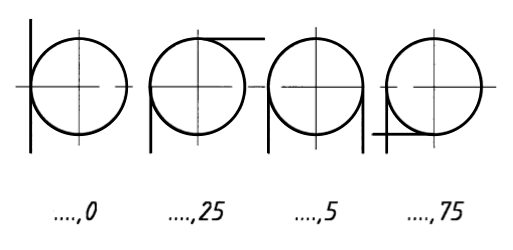
\includegraphics[width=0.75\linewidth]{federn/drehfedern-winkel}
		\end{figure}
\end{eeqn}

% Gesamtlänge Federkörper
\begin{eeqn}{Gesamtlänge Federköper}
	Bei anliegenden Windungen:
	\begin{align}
		L_\text{K} &= (i_\text{F}+1,5)\cdot d
	\end{align}
	Bei Windungsabstand:
	\begin{align}
		L_\text{K} &= i_\text{F} \cdot (a+d) +d
	\end{align}
\end{eeqn}

\pagebreak
\subsection{Drehstabfedern}
\begin{vardef}
	\item[$l_\text{k}$] Kopflänge
	\item[$l_\text{f}$] federnde Länge (Länge eines reinen Torsionsstab, der die selbe Federwirkung hätte)
	\item[$l_\text{h}$] Hohlkehlenlänge
	\item[$l_\text{e}$] Ersatzlänge 	
	\item[$l_\text{k}$] Kopflänge
	\item[$d$] Durchmesser im federnden Bereich
\end{vardef}
\begin{figure}[H]
	\centering
	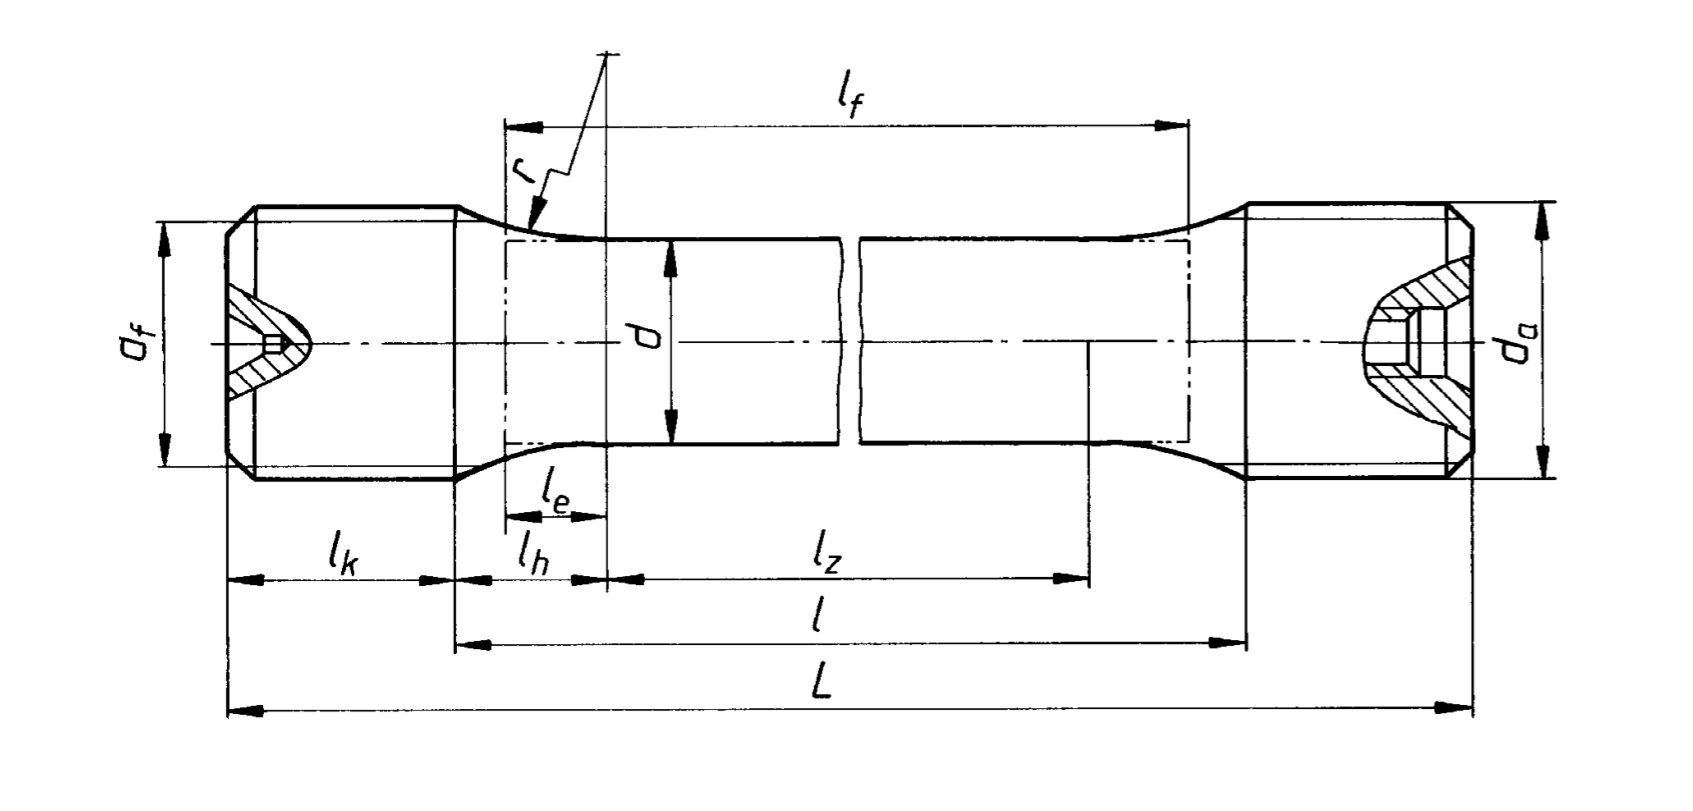
\includegraphics[width=0.8\linewidth]{federn/drehstabfeder}
	\caption*{Drehstabfeder}
\end{figure}

\hrule
% Federgeometrie
\begin{eeqn}{Federgeometrie}
	\begin{align}
		& l_\text{h} = \frac{d_\text{f}-d}{2}\cdot \sqrt{\frac{4r}{d_\text{f}-d}-1} \\
		& l_\text{z} = l- 2\cdot l_\text{h} \\
		& l_\text{e} = \nu \cdot l_\text{h}\\
		& l_\text{f} = l_\text{z} + 2\cdot l_\text{e}
	\end{align}
\end{eeqn}

% Federrate
\begin{eeqn}{Federrate}
	\begin{align}
		c &= \frac{M_\text{t}}{\alpha} = \frac{G\cdot I_\text{p}}{l_\text{f}}
		\intertext{Der Winkel ist in \textbf{rad}, zum umrechnen nutze:}
		[Grad] &= [rad] \cdot \frac{360}{2 \pi}
	\end{align}
\end{eeqn}

% Auslegung der Feder
\begin{eeqn}{Auslegung der Feder}
	Die maximale Belastung der Feder ergibt sich aus der maximalen Torsionsspannung, die aus der Verdrillung resultiert.
	\begin{align}
		M_\text{max} &= \tau_\text{zul} \cdot \frac{\pi \cdot d^3}{16}
	\end{align}
\end{eeqn}

\subsection{Schraubenfedern (Zug-/Druckfedern)}
\begin{vardef}
	\item[$s^*$] Federweg pro Windung
	\item[$s$] Federweg der gesamten Feder 
	\item[$d$] Drahtdurchmesser
	\item[$D_\text{m}$] Mittlerer Durchmesser der Feder
	\item[$S_\text{a}$] Restspielsumme (Sicherheitsabstand)
	\item[$i_\text{s}$] Anzahl der eingerollten oder eingeschraubten Windungen
	\item[$L_\text{c}$] Blocklänge der Feder (Alle Windungen liegen aufeinander)
	\item[$L_\text{n}$] Nennlänge der Feder (minimale Federlänge)
	\item[$i_\text{G}$] Gesamtwindungszahl
	\item[$i_\text{F}$] Anzahl federnder Windungen
\end{vardef}

\hrule
% Federgeometrie
\begin{eeqn}{Federgeometrie}
	\vspace{5pt} siehe \ref{sec:federgeometrie-drehfedern} auf Seite \pageref{sec:federgeometrie-drehfedern}
\end{eeqn}

% Federrate
\begin{eeqn}{Federrate}
	\begin{align}
		c &= \frac{G \cdot d^4}{8\cdot i_\text{F} \cdot D_\text{m}^3}
	\end{align}
\end{eeqn}

% Federkraft
\begin{eeqn}{Federkraft}
	\begin{align}
		F &= c \cdot s \qquad \text{$s$ ist der Federweg} 
	\end{align}
\end{eeqn}

% Federweg
\begin{eeqn}{Federweg}
	\begin{align}
		& s^* = \frac{8\cdot F \cdot D_\text{m}^3}{G\cdot d^4} \\
		& s = i_\text{F} \cdot s^*
	\end{align}
\end{eeqn}

% Wicklungsverhältnis
\begin{eeqn}{Wicklungsverhältnis}
	\begin{align}
		W &= \frac{D_m}{d}
	\end{align}
\end{eeqn}

% Korrekturfaktor
\begin{eeqn}{Korrekturfaktor durch Spannnungserhöhungen an der Innenseite}
	\begin{align}
		q & = \frac{W+0,5}{W-0,75}
	\end{align}
	Beim Auslegen von Federn wird $q=1$ gesetzt, später wird dann der tatsächliche Wert von $q$ bestimmt.
\end{eeqn}

\enlargethispage{\baselineskip}

% Spannungen in der Feder
\begin{eeqn}{Spannungen in der Feder}
	Alle Spannungen in der Feder ausschließlich durch Torsion:
	\begin{align}
		\tau_\text{t} &= q \cdot \frac{8 \cdot F \cdot  D_\text{m}}{\pi \cdot d^3}
	\end{align}
	Das in diesem Belastungsfall wirkende Moment ergibt sich aus:
	\begin{align}
		M_\text{t} &= F \cdot \frac{D_\text{m}}{2}
	\end{align}
\end{eeqn}

% Kaltgeformte Druckfedern
\begin{eeqn}{Kaltgeformte Druckfedern}
	\begin{align}
		& i_\text{g} = i_\text{f} +2 \\
		& S_\text{a} = i_\text{f}\cdot \left(0,0015\cdot \frac{D_\text{m}^2}{d}+0,1\cdot d\right)\\
		& L_\text{n} = L_\text{C} + S_\text{a}\\
		\intertext{angelegte Enden:}
		& L_\text{C} = (i_\text{g}+1,5) \cdot d
		\intertext{angelegte und plangeschliffene Enden:}
		& L_\text{C} = i_\text{g} \cdot d
		\intertext{ungespannte Länge der Feder:}
		& L_0 = L_n + \frac{F}{c} \\ 
		\intertext{man braucht $F$ zum erreichen der minimalen Nennlänge}
		\intertext{Blockkraft:}
		& F_c = F + c \cdot S_a \\  
		\intertext{man braucht $F$ zum erreichen der minimalen Nennlänge}
	\end{align}
\end{eeqn}

% Warmgeformten Druckfedern
\begin{eeqn}{Warmgeformte Druckfedern}
	\begin{align}
		& i_\text{g} = i_\text{f} +1,5 \\
		& S_\text{a} = 0,02 \cdot D_\text{a} \cdot i_\text{f} 
		\intertext{angelegte Enden:}
		& L_\text{C} = (i_\text{g}+1,1) \cdot d
		\intertext{angelegte und plangeschliffene Enden:}
		& L_\text{C} = (i_\text{g}-0,3) \cdot d
	\end{align}
\end{eeqn}


% Warmgeformten Zugfedern
\begin{eeqn}{Warmgeformte Zugfedern}
	abgebogene Ösen:
	\begin{align}
		& i_\text{g} = i_\text{f} \\
		& L_\text{C} = (i_\text{g}+1) \cdot d
	\end{align}
	eingerollt oder eingeschraubte Enden:
	\begin{align}
		i_\text{g} = i_\text{f} + i_\text{s}
	\end{align}
	Ösen:
	\begin{align}
		\text{Parallel} &\quad i_\text{f} = x,0~\text{oder}~x,5 \\ 
		\text{Versetzt} &\quad i_\text{f} = x,25~\text{oder}~x,75	\end{align}
\end{eeqn}

	\section{Schraubenverbindungen}
\begin{vardef}
	\item[$P$] Steigung in mm (Höhenunterschied bei einem Umlauf)
	\item[$\alpha$] Windungssteigungswinkel
	\item[$\beta$] Flankenöffnungswinkel (bei metrischen Schrauben $\beta=60\degree$)
	\item[$d_2$] mittlerer Flankendruchmesser
	\item[$d_3$] Kerndurchmesser
	\item[$d$] Nenndruchmesser (Gewindeaußendruchmesser)
	\item[$d_\text{K}$] Kopfdruchmesser (=Schlüsselweite)
	\item[$D_\text{B}$] Bohrungsdurchmesser (Da wo die Schraube rein soll, am besten kleiner als Kopfdurchmesser)
	\item[$r_\text{A}$] Mittlerer belasteter Durchmesser des Schraubenkopfs
	\item[$A_\text{K}$] Schraubenkopfauflagefläche
	\item[$A_\text{S}$] gefährdeter Spannungsquerschnitt der Schraube (tabelliert)
	\item[$\varrho'$] Winkel des Reibungskegels
	\item[$\mu$] Reibungskoeffizient
	\item[$c_\text{s}$] Federrate der Schraube
	\item[$c_\text{p}$] Federrate der Zwischenlage
	\item[$\Phi$] Kraftverhältnis
	\item[$\Phi_\text{n}$] Kraftverhältnis unter Berücksichtigung des Krafteinleitungsfaktor
	\item[$F_\text{KL}$] Klemmkraft (Kraft in der Verbindungsfuge)
	\item[$F_\text{A}$] Axiale Betriebskraft (Kraft, die die verbundenen Teile auseinander zieht; immer Zugkraft!)
	\item[$F_\text{S}$] Schraubenkraft (Kraft in der Schraube, die die Schraube dehnt)
	\item[$F_\text{SA}$] Schraubenzusatzkraft	\item[$F_\text{PA}$] Kraft der Zwischenlage
	\item[$F_\text{VM}$] Montagevorspannkraft
	\item[$F_\text{z}$] Vorspannkraftverlust durch Setzerscheinung
	\item[$f_\text{z}$] Setzbetrag
	\item[$M_\text{G}$] Moment am Gewinde
	\item[$M_\text{K}$] Moment am Kopf
	\item[$M_\text{A}$] Anziehmoment
	\item[$n$] Krafteinleitungsfaktor
	\item[$\alpha_\text{A}$] Anziehfaktor (Unschärfe bei der Montage der Schraube)
\end{vardef}

% Windungssteigungswinkel
\hrule
\begin{eeqn}{Windungs\-steigungs\-winkel}
	\begin{align}
	\alpha &= \arctan{\left(\frac{P}{\pi \cdot d_2}\right)}
	\end{align}
\end{eeqn}

% Reibungswinkel
\begin{eeqn}{Reibungs\-winkel}
	\begin{align}
	\varrho' &= \arctan{\left(\frac{\mu}{\cos{\left(\frac{\beta}{2}\right)}}\right)}
	\end{align}
\end{eeqn}

% Kraftverhältnis
\begin{eeqn}{Kraftverhältnis}
	\begin{align}
		\Phi & = \frac{c_\text{s}}{c_\text{s}+c_\text{p}}
	\end{align}
	Wenn die Krafteinleitungstiefe berücksichtigt wird (immer im Zusammenhang mit $F_\text{A}$)
	\begin{align}
		\Phi_\text{n} & = \frac{c_\text{s}}{c_\text{s}+c_\text{p}} \cdot n
	\end{align}
\end{eeqn}

% Kopfgeometrie
\begin{eeqn}{Geometrie des Schraubenkopfs}
	\begin{align}
		& r_\text{A} = \frac{d_\text{K}+D_\text{B}}{4} \\
		& A_\text{K} = \frac{\pi}{4} \cdot (d_\text{k}^2-D_\text{B}^2)
	\end{align}
	Es muss auf eventuelle Fasen an der Bohrung geachtet werden, der Bohrungsdurchmesser $D_\text{B}$ vergrößert sich entsprechend.
\end{eeqn}

% Wirkungsgrad
\begin{eeqn}{Wirkungsgrad}
	\begin{align}
		\eta & = \frac{\tan \alpha}{\tan(\alpha + \varrho')}
	\end{align}
\end{eeqn}

% Setzkraftverlust in der Schraube
\begin{eeqn}{Setzkraftverlust}
	\begin{align}
		& F_\text{Z} = f_\text{z} \cdot c_\text{p} \cdot \Phi
	\end{align}
	Durch Mikroplastizitäten in den Kontaktflächen der Verbindung findet eine Entlastung der selbigen statt. 
\end{eeqn}

% Montagevorspannkraft
\begin{eeqn}{Montagevorspannkraft}
	\begin{align}
		& F_\text{VM,min} = F_\text{KL} + F_\text{A}\cdot (1-\Phi_\text{n})+F_\text{Z} \\
		& F_\text{VM} = \alpha_\text{A}\cdot F_\text{VM,min}
	\end{align}
\end{eeqn}

% Moment zum Lösen der Schraube
\begin{eeqn}{Moment zum Lösen der Schraube}
	\begin{align}
		& F_\text{S} = F_\text{KL} + F_\text{A}\cdot (1-\Phi_\text{n}) \\
		& M_\text{Lös} = F_\text{s} \cdot \tan (\alpha - \varrho') \cdot \frac{d_2}{2}
	\end{align}
	Moment am Gewinde ohne den Anteil des Setzbetrags
\end{eeqn}

% Moment am Kopf
\begin{eeqn}{Moment am Kopf}
	\begin{align}
		M_\text{K} & = F_\text{VM} \cdot \mu \cdot r_\text{A}
	\end{align}
\end{eeqn}

% Moment am Gewinde
\begin{eeqn}{Moment am Gewinde}
	\begin{align}
		& M_\text{G} = F_\text{VM} \cdot \frac{d_2}{2} \cdot \tan{(\alpha+\varrho')}
	\end{align}
\end{eeqn}

% Anziehmoment
\begin{eeqn}{Anziehmoment}
	\begin{align}
		& M_\text{A} = M_\text{K} + M_\text{G}
	\end{align}
\end{eeqn}


% Pressung am Kopf der Schraube
\begin{eeqn}{Pressung am Kopf der Schraube}
	\begin{align}
		P &= \frac{F_\text{VM}+F_\text{A}\cdot\Phi_\text{n}}{A_\text{K}}
	\end{align}
\end{eeqn}

% Spannugen in der Schraube
\begin{eeqn}{Spannungen in der Schraube}
	\begin{align}
		\sigma_\text{v} &= \sqrt{\left(\frac{F_\text{VM}+F_\text{SA}}{A_\text{S}}\right)^2+3\cdot \left(\frac{16 \cdot M_\text{G}}{\pi \cdot d_3^3}\right)^2} \label{eqn:spannungen_schraube}
	\end{align}
	Es gilt $F_\text{SA} = F_\text{A}\cdot \Phi_\text{n}$. Die erhaltenen Vergleichsspannung muss kleiner sein als die Streckgrenze $R_\text{e}$ der Schraube. Diese ergibt sich aus den Festigkeitsangaben der Schraube bzw. Mutter. Die Bezeichnung lautet immer $x.y$ wobei $x=R_\text{m}/100$ und $y=R_\text{e}/R_\text{m}$ (es ist immer $y < 1$). Es gilt:
	\begin{align}
		R_\text{e} &= x \cdot 100 \cdot y ~\text{N/mm}^2
	\end{align}
\end{eeqn}

% dynamisch belastete Schrauben
\begin{eeqn}{dynamisch belastete Schrauben}
	\begin{enumerate}[itemsep=0mm,leftmargin=12pt]
	\item Berechnung der Schraubenzusatzkräfte für beide Amplituden ($F_\text{SA,1}$, $F_\text{SA,1}$):
	\begin{align}
		F_\text{SA} &= F_\text{A}\cdot \Phi_\text{n}
	\end{align}
	\item Berechnung der Mittelspannung $\sigma_\text{v}$ mit der größeren Schraubenzusatzkraft gemäß Formel \ref{eqn:spannungen_schraube}.
	\item Ermitteln der mittlere Schraubenzusatzkraft $F_\text{SA,m}$:
	\begin{align}
		F_\text{SA,m} &= \frac{F_\text{SA,1} + F_\text{SA,2}}{2}
	\end{align}
	Diese ergibt mit dem Spannungsquerschnitt die Ausschlagsspannung $\sigma_\text{a}$:
	\begin{align}
		\sigma_\text{a} &= \frac{F_\text{SA,m}}{A_\text{S}}
	\end{align}
	\item Im Betriebszustand pendelt die Spannung um $\pm \sigma_\text{a}$ und hat die Mittelspannung $\sigma_{v}$.
	\end{enumerate}
	Umso kleiner $\Phi_\text{n}$ ist, desto besser ist die Schraubverbindung für dynamische Belastungen geeignet (Die Ausschlagsspannugen sind kleiner bei kleinem $\Phi_\text{n}$).
	Es gilt die Römerformel $\sigma_\text{a} \le 0,07 \cdot R_\text{E}$, ist diese Bedingung nicht erfüllt, müssen entweder mehr Schrauben verwendet werden oder der Faktor $\Phi_\text{n}$ verkleinert werden. \\
\end{eeqn}

\begin{figure}[H]
	\centering
	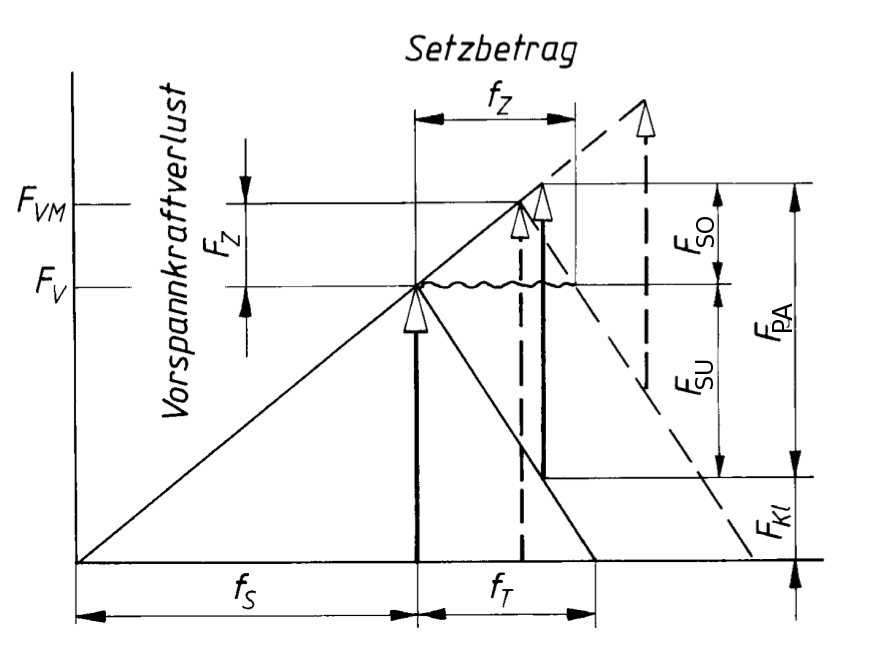
\includegraphics[width=0.8\linewidth]{schrauben/schraubendiagramm}
	\caption*{Schraubendiagramm einer dynamisch belasteten Schraube mit Setzerscheinung}
\end{figure}


% Auslegung von Schrauben
\hrule
\begin{eeqn}{Auslegung von Schrauben}
	\begin{enumerate}[itemsep=0mm,leftmargin=12pt]
		\item Wahl der Festigkeitsklasse (wenn nicht anders angegeben: 8.8 / $R_\text{e}=\SI{640}{N/mm^2}$) und errechnen von $R_\text{e}$.
		\item Ermittlung der zulässigen Spannung gemäß der Römerformel ($\mu_\text{Stahl}=0,15$):
			\begin{align}
				\sigma_\text{zul} &= (0,85-\mu)\cdot R_\text{e}
			\end{align}
		\item Bestimmung des Spannungsquerschnitts bei gegebener Schraubenkraft $F_\text{S}=F_\text{KL}+F_\text{A}$ (Beim Auslegen gilt, wenn nichts anderes angegeben: $F_\text{A}=0$; $\alpha_\text{A}=1$):
			\begin{align}
				A_\text{S} &\geq \frac{\alpha_\text{A} \cdot F_\text{S}}{\sigma_\text{zul}}
			\end{align}
		\item Aus Tabellen kann mit dem gefundenen Spannungsquerschnnitt eine Schraube ausgewählt werden. Mit der gewählten Schraube sollten Pressung und Spannungen überschlagsmäßig überprüft werden, hierfür muss zunächst die Schraubenauflagefläche $A_\text{K}$ berechnet werden.
	\end{enumerate}
\end{eeqn}
	\section{Passfedern und Keilwellen}
\subsection{Passfedern}
\begin{vardef}
	\item[$d$] Wellendruchmesser
	\item[$b$] Passfederbreite
	\item[$h$] Passfederhöhe
	\item[$t_1$] Nuttiefe Welle
	\item[$t_2$] Nuttiefe Narbe
	\item[$P_\text{N}$] Pressung zwischen Passfeder und Narbe
	\item[$P_\text{W}$] Pressung zwischen Passfeder und Welle
	\item[$l$] Gesamtlänge der Passfeder
	\item[$l_\text{tr}$] tragende Länge der Passfeder
	\item[$\varphi$] Lastverteilungsfaktor (wie gleichmäßig werden die Passfedern belastet)
	\item[$n$] Anzahl der Passfedern
	\item[$F_\text{u}$] Umfangskraft
	\item[$M$] Moment auf die Welle
\end{vardef}

\hrule
% Beanspruchung der Narbe
\begin{eeqn}{tragende Länge}
	\begin{align}
		&\text{rundstrinige Passfedern:}&\quad l &= l_\text{tr}+b \\
		&\text{gradstirnige Passfedern:}&\quad l &= l_\text{tr}
	\end{align}
\end{eeqn}	

% Pressung der Narbe auf die Passfeder
\begin{eeqn}{Pressung der Narbe auf die Passfeder}
	Wenn $l_\text{tr} \leq 1,5 \cdot d$:
	\begin{align}
		P_\text{N} &= \frac{2\cdot M}{(h-t_1) \cdot l_\text{tr} \cdot d}
	\end{align}
	$t_1$ aus Tabelle
\end{eeqn}	

% Pressung der Narbe auf die Passfeder
\begin{eeqn}{Pressung der Welle auf die Passfeder}
	Wenn $l_\text{tr} \leq 1,5 \cdot d$:
	\begin{align}
		P_\text{W} &= \frac{2\cdot M}{d\cdot l_\text{tr} \cdot t_1}
	\end{align}
	Es gilt der Grundsatz, dass Passfedern normalerweise auf die Belastungen in der Narbe ausgelegt werden. 
\end{eeqn}

\enlargethispage{\baselineskip}

% Mehrere Passfedern
\begin{eeqn}{mehrere Passfedern}
	Wenn $l_\text{tr} \leq 1,5 \cdot d$:
	\begin{align}
		P_\text{N} &= \frac{2\cdot M}{(h-t_1)\cdot l_\text{tr} \cdot d \cdot \varphi \cdot n}
	\end{align}
	Für den Lastverteilungsfaktor gilt:
	\begin{align*}
		&n =2~: \quad \varphi =0,75\\
		&n =3~: \quad \varphi =0,6\\
	\end{align*}
	Der Term $n \cdot \varphi$ konvergiert gegen den Wert 2. Die Erhöhung der Anzahl der Passfedern ist deshalb wenig effizient, wenn die tragende Länge $l_\text{tr}$ reduziert werden soll.
\end{eeqn}

% Scherung in der Passfeder
\begin{eeqn}{Scherung in der Passfeder}
	\begin{align}
		\tau_\text{a} &= \frac{F_\text{u}}{b\cdot l_\text{tr}} = \frac{2\cdot M}{d\cdot b \cdot l_\text{tr}}
	\end{align}
	In der Regel ist die Berechnung der Scherspannung nicht erforderlich, da die wirkenden Pressungen viel größere sind.
\end{eeqn}

\subsection{Keilwellenverbindung}
\begin{vardef}
	\item[$h'$] tragende Höhe (Anteil der Höhe der Flanken, die die Drehmomente übertragen)
	\item[$D$] Außendurchmesser der Keilwelle
	\item[$d$] Innendurchmesser der Keilwelle
	\item[$d_\text{m}$] Mittlerer Durchmesser der Keilwelle
	\item[$L$] Verzahnte Länge der Keile
	\item[$n$] Anzahl der Flanken
\end{vardef}

\hrule
% tragende Höhe
\begin{eeqn}{tragende Höhe}
	\begin{align}
		h' = 0,4 \cdot (D-d)
	\end{align}
\end{eeqn}

% mittlerer Durchmesser
\begin{eeqn}{Mittlerer Durchmesser}
	\begin{align}
		d_\text{m} &= \frac{D+d}{2}
	\end{align}
\end{eeqn}

% Auf die Keile wirkende Pressung
\begin{eeqn}{Auf die Keile wirkende Pressung}
	\begin{align}
		P &= \frac{2\cdot M}{d_\text{m} \cdot h' \cdot L \cdot n \cdot \varphi}
	\end{align}
	Für den Lastverteilungsfaktor gilt:
	\begin{align*}
		&\text{Flankenzentrierung}: \quad &\varphi &=0,9\\
		&\text{Innenzentrierung}: \quad &\varphi &=0,75\\
	\end{align*}
\end{eeqn}

	\section{Bolzen- und Stiftverbindungen}
\subsection{Stiftverbindungen}
\begin{figure}[H]
	\centering
	\begin{minipage}[b]{0.22\linewidth}
		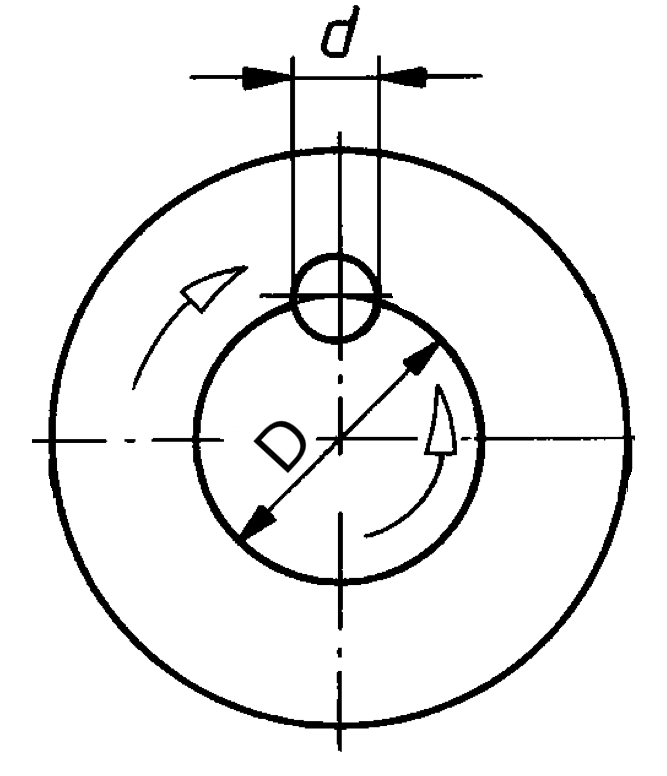
\includegraphics[width=\linewidth]{bolzen-und-stiftverbindungen/laengststift}
		\caption*{Längsstift}
	\end{minipage}
	\begin{minipage}[b]{0.22\linewidth}
		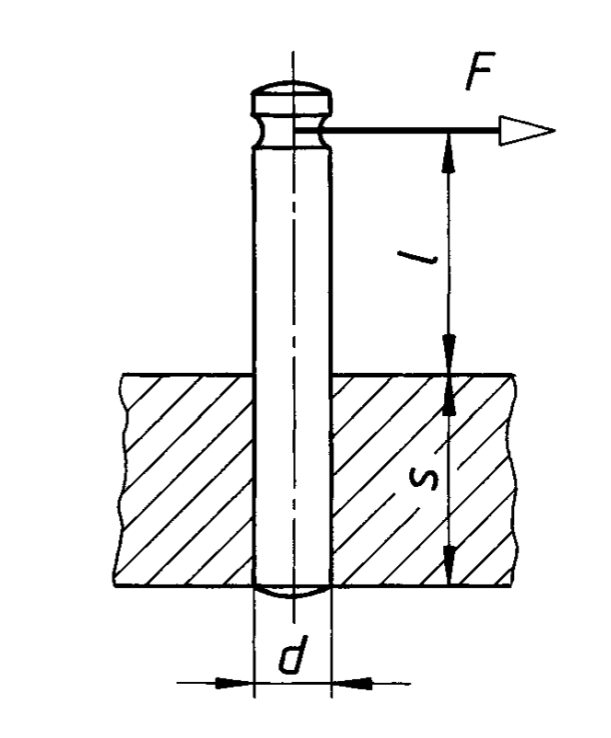
\includegraphics[width=\linewidth]{bolzen-und-stiftverbindungen/steckstift}
		\caption*{Steckstift}
	\end{minipage}
	\begin{minipage}[b]{0.22\linewidth}
		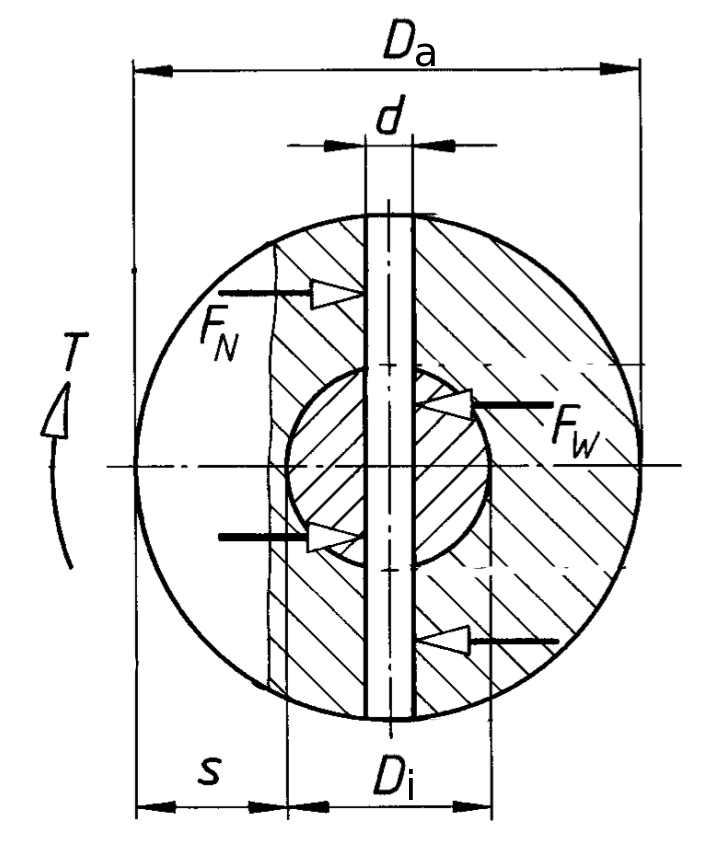
\includegraphics[width=\linewidth]{bolzen-und-stiftverbindungen/querstift}
		\caption*{Querstift}
	\end{minipage}
\end{figure}

% Längststiftverbindungen
\begin{eeqn}{Längsstiftverbindung}
	\begin{align}
		& P = \frac{4\cdot M}{L \cdot D \cdot d}\\
		& \tau_\text{A} = \frac{2\cdot M}{L \cdot D \cdot d}
	\end{align}
\end{eeqn}

% Steckstiftverbindung
\begin{eeqn}{Steckstiftverbindung}
	\begin{align}
		P_\text{max} &= \frac{2\cdot F}{d \cdot s}\cdot \left(3 \cdot \frac{l}{s}+2\right) + P_\text{Montage}
	\end{align}
	Maximale Pressung einer Steckstiftverbindung, die im Sitz zu erwarten ist. \\
	Beanspruchung des Stifts:
	\begin{align}
		&\tau_\text{A} = \frac{F}{A} = \frac{4\cdot F}{\pi \cdot d^2}\\
		&\sigma_\text{B} = \frac{M_\text{B}}{W_\text{ax}} = \frac{32\cdot F \cdot l}{\pi \cdot d^3}
 	\end{align}
 	Wenn beide Enden des Steckstifts versenkt sind, gilt (siehe Aufgabe 44):

	\begin{align}
		P &= \frac{F}{d\cdot s} \\
		\sigma_\text{B} &= \frac{M_\text{B}}{W_\text{ax}} = \frac{32\cdot F \cdot s}{\pi \cdot d^3 \cdot 2}
	\end{align}
\end{eeqn}



% Querstiftsverbindung
\begin{eeqn}{Querstiftsverbindung}
	Wenn auf die Welle das Moment $M$ wirkt, entsteht in der Narbe die Pressung $P_\text{N}$ und in der Welle die Pressung $P_\text{W}$:
	\begin{align}
		& P_\text{N} = \frac{4\cdot M}{d\cdot(D_\text{a}^2-D_\text{i}^2)} \\
		& P_\text{W} = \frac{6\cdot M}{d \cdot D_\text{i}^2}
	\end{align}
	Der Stift erleidet Scherspannungen:
	\begin{align}
		\tau_\text{A} &= \frac{4\cdot M}{\pi \cdot d^2 \cdot D_\text{i}}
	\end{align}
\end{eeqn}

\subsection{Bolzenverbindungen}
\begin{figure}[H]
	\centering
	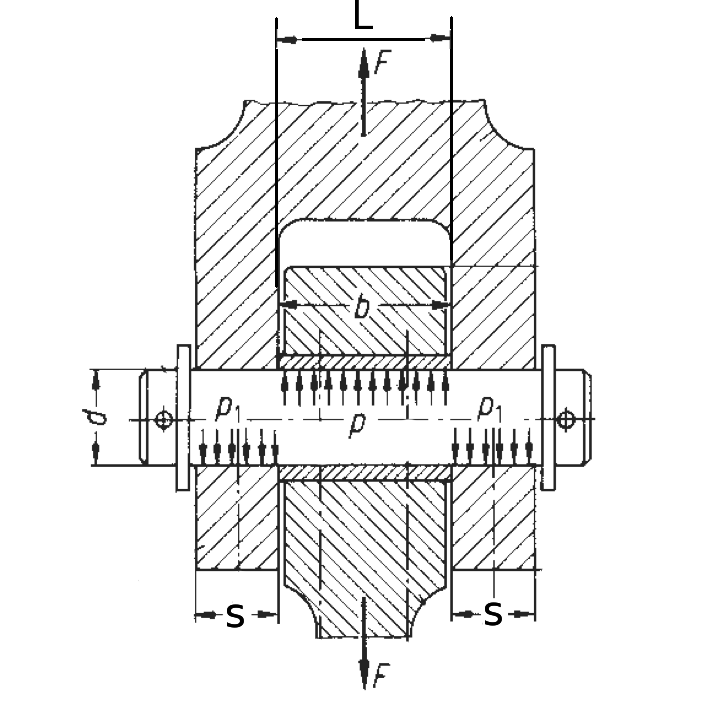
\includegraphics[width=0.7\linewidth]{bolzen-und-stiftverbindungen/bolzen}
	\caption*{Gabel-Welle Verbindung mit einem Bolzen}
\end{figure}
\vfill
\pagebreak
\hrule
% Biegemomente in Gabel Stange Verbindungen
\begin{eeqn}{Biegemomente in Gabel-Stange Verbindungen}
	\begin{table}[H]
		\centering
		\caption*{Unterschiedliche Passungsverhältnisse für Gabel-Stange Verbindungen}
		\begin{tabularx}{\linewidth}{llX}
			\toprule
			Passung Gabel & Passung Stange & $M_\text{B}$ \\
			\midrule
			Spiel & Spiel & $\displaystyle\frac{F\cdot (L+2\cdot s)}{8}$ \\[3mm]
			Pressung & Spiel & $\displaystyle\frac{F \cdot L}{8} $ \\[3mm]
			Spiel & Pressung & $\displaystyle\frac{F\cdot s}{4} $ \\
			\bottomrule
		\end{tabularx}
	\end{table}
\end{eeqn}

\begin{eeqn}{Gabel-Stange Verbindung}
	Zwischen Bolzen und Stange wirkt die Pressung $P_\text{Stange}$:
	\begin{align}
		P_\text{Stange} &= \frac{F}{L\cdot d}
	\end{align}
	Zwischen Bolzen und Gabel wirkt die Pressung $P_\text{Gabel}$:
	\begin{align}
		P_\text{Gabel} &= \frac{F}{2 \cdot s \cdot d}
	\end{align}
	Die Montagepressung $P_\text{Montage}$ wird beim auf Pressung beanspruchtem Element addiert.
	Der Bolzen erleidet Scher- und Biegespannungen:
	\begin{align}
		& \tau_\text{A} = \frac{2\cdot F}{\pi \cdot d^2} \\
		& \sigma_\text{B} = \frac{32\cdot M_\text{B}}{\pi \cdot d^3}
	\end{align}
\end{eeqn}

% Beanspruchung der Gabel
\begin{eeqn}{Beanspruchung der Gabel}
	Wenn auf einen Bolzen, der in einer Gabel gelagert ist, eine radiale Betriebskraft $F$ wirkt, entsteht in der Gabel eine Zugbeanspruchung $\sigma_\text{z}$:
	\begin{align}
		\sigma_\text{z} &= \frac{F}{A} = \frac{F}{2\cdot s\cdot (D-d)}
	\end{align}
	Hierbei hat die Gabel den Durchmesser $D$ und eine Dicke $s$. Der Bolzen hat den Durchmesser $d$. 
\end{eeqn}
	\section{Kupplungen}

\subsection{Einscheibenkupplungen}
\begin{vardef}
	\item[$R_\text{a}$] Außenradius der Kupplungsscheibe
	\item[$R_\text{i}$] Innenradius der Kupplungsscheibe
	\item[$S$] Axiale Betriebskraft
	\item[$d_\text{m}$] Mittlerer Durchmesser der Kupplungsscheibe
	\item[$b$] Breite der Kupplungsscheibe
\end{vardef}

\begin{figure}[H]
	\centering
	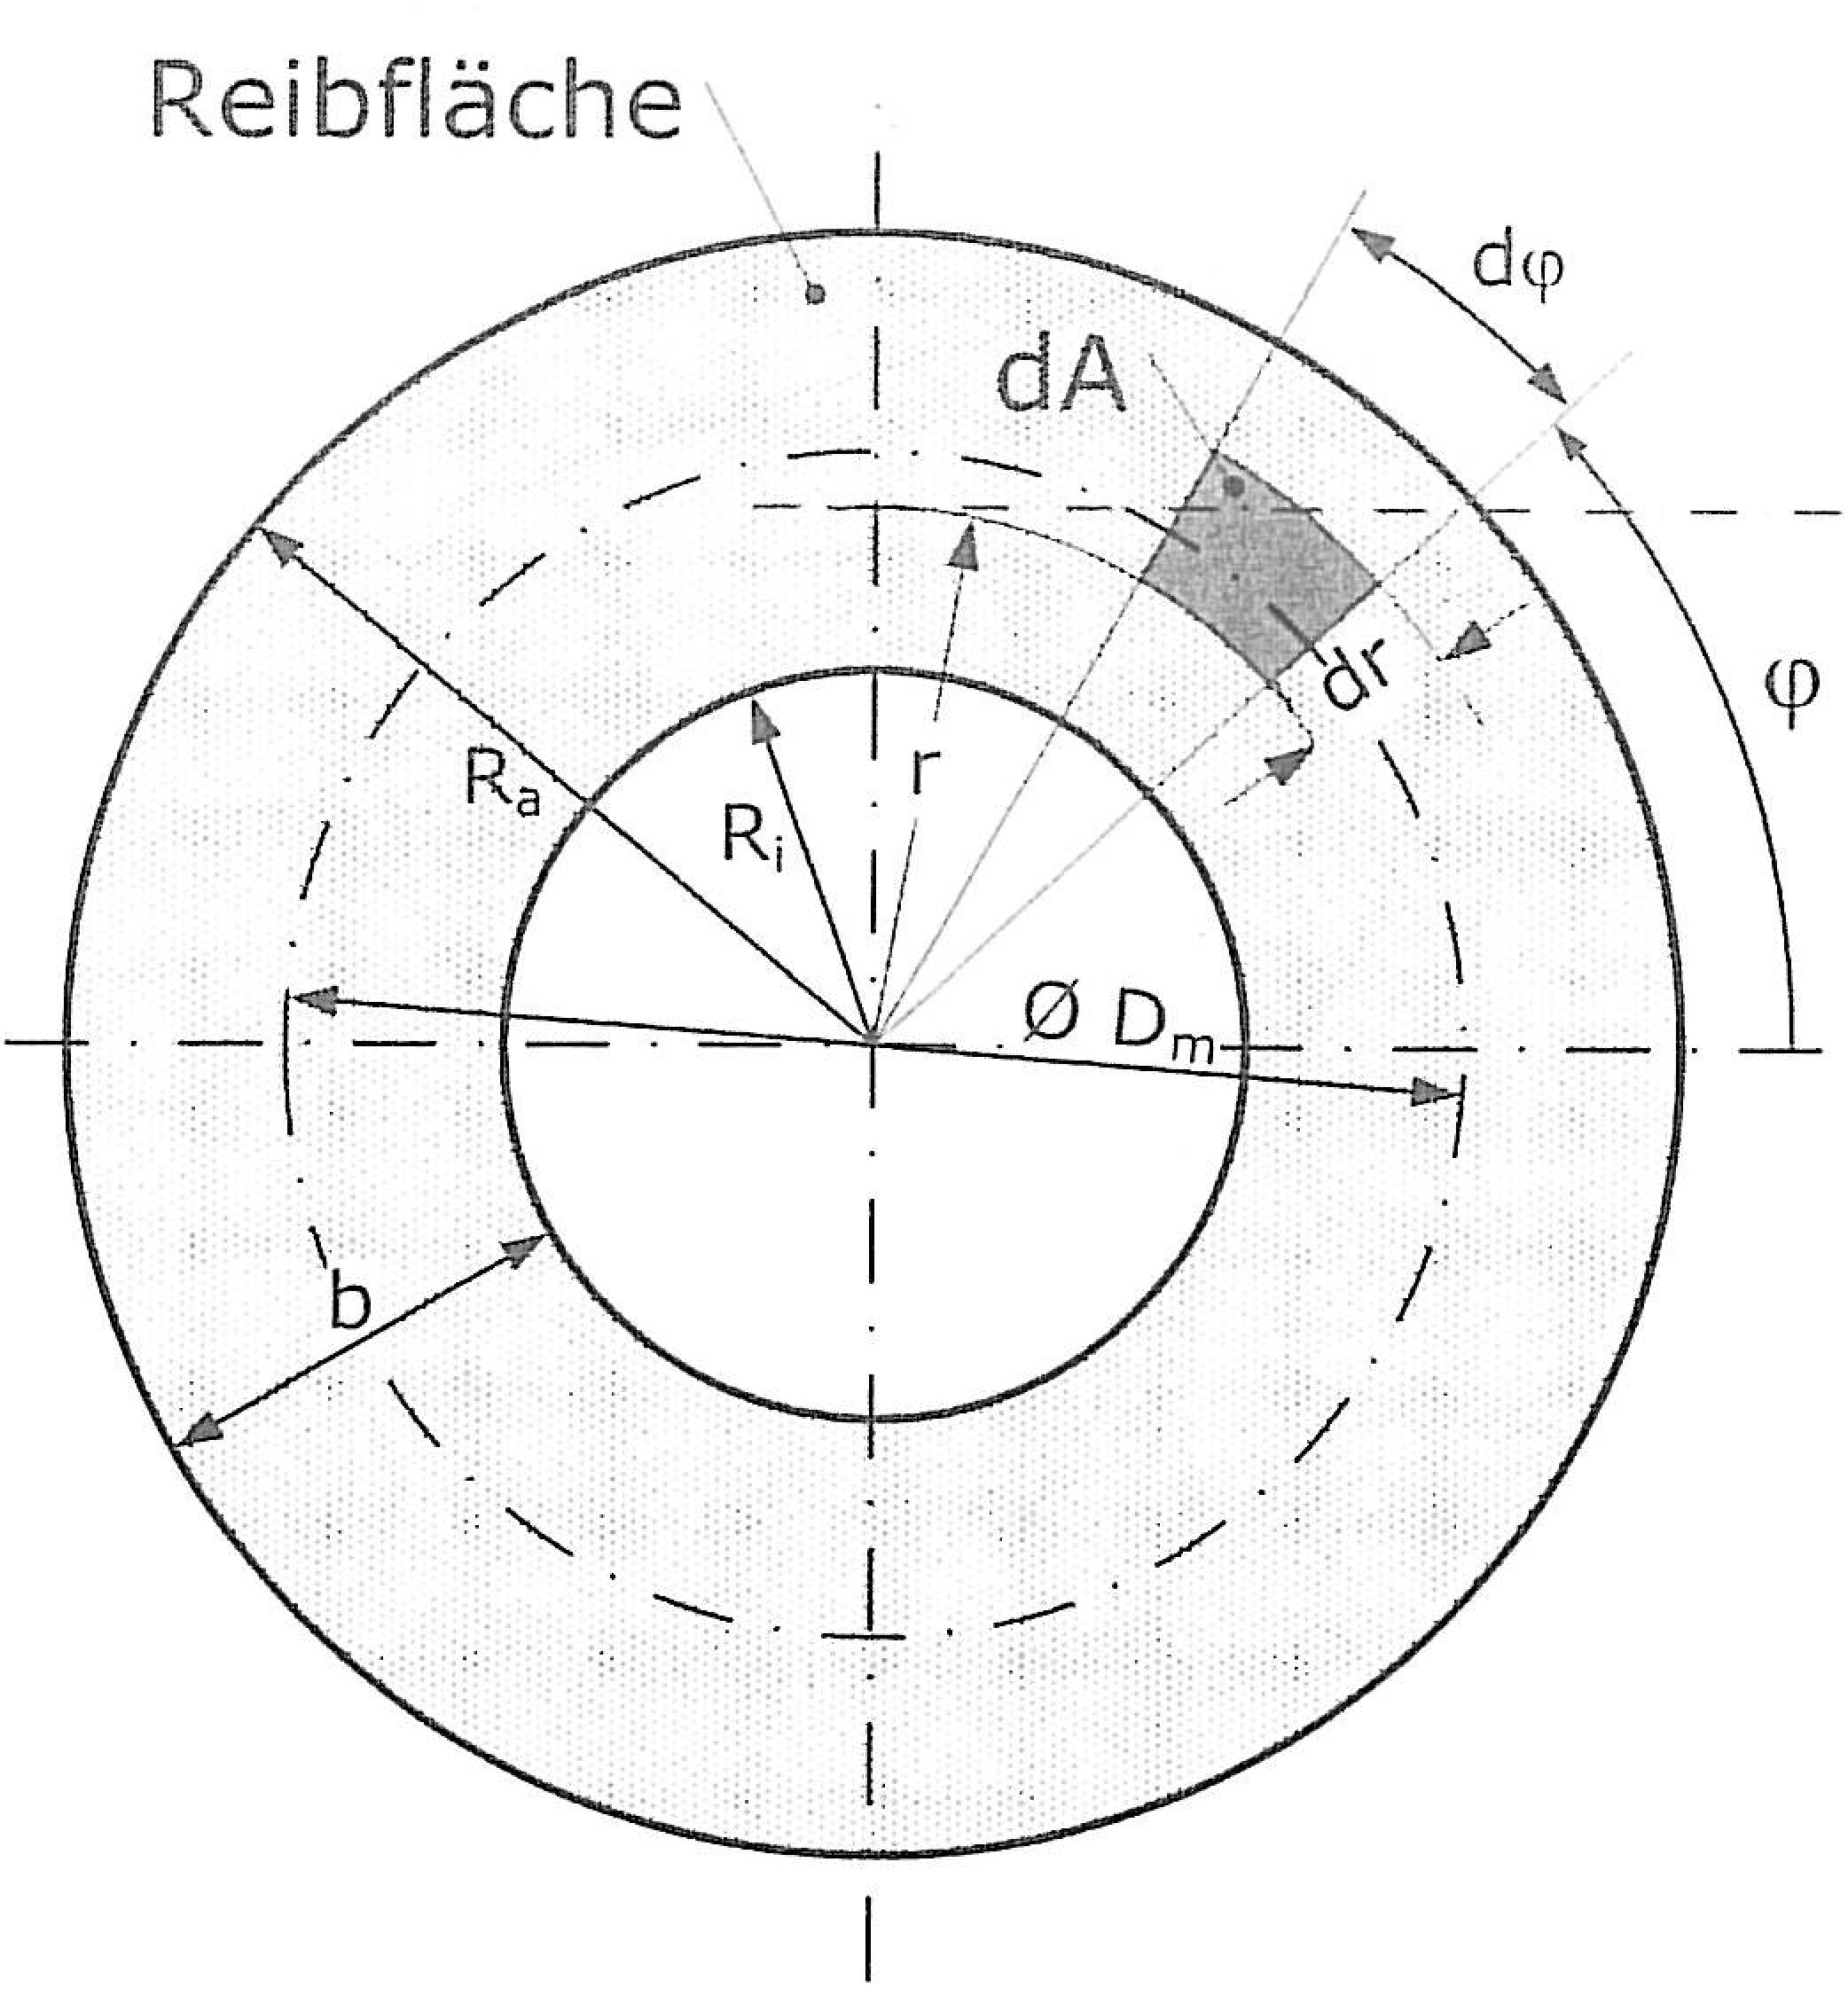
\includegraphics[width=0.35\linewidth]{kupplungen/einscheibenkupplung.jpg}
	\caption*{Geometrie der Kupplung}
\end{figure}

% Hilfsgrößen
\hrule
\begin{eeqn}{Hilfsgrößen}
	\begin{align}
		&b = \frac{D_\text{a}-D_\text{i}}{2} = R_\text{a} - R_\text{i}  \\
		&d_\text{m} = \frac{D_\text{A}+D_\text{i}}{2} =R_\text{a} + R_\text{i}
	\end{align}
\end{eeqn}

% Moment im Neuzustand der Kupplung
\begin{eeqn}{Moment im Neuzustand der Kupplung}
	\begin{align}
		M &= \frac{2\cdot S \cdot \mu}{3 \cdot d_\text{m} \cdot b} \cdot \left( R_\text{a}^3 - R_\text{i}^3\right)
	\end{align}
\end{eeqn}

% Moment im Gebrauchtzustand der Kupplung
\begin{eeqn}{Moment im Gebrauchtzustand der Kupplung}
	\begin{align}
		M &= S \cdot \mu \cdot \frac{d_\text{m}}{2}
	\end{align}
\end{eeqn}

% Auslegung von Kupplungen
\begin{eeqn}{Auslegung von Kupplungen}
	Kupplungen werden immer auf den Gebrauchtzustand ausgelegt, anschließend wird dann das Moment im Neuzustand überprüft. \\
	Wenn bei der Kupplung $N$ Reibflächen entstehen, gilt für das gesamte übertragbare Moment $M_\text{zul}$:
	\begin{align}
		M_\text{ges} = N \cdot M
	\end{align}
\end{eeqn}

\subsection{Kegelpressverbindungen}
\begin{vardef}
	\item[$\beta$] Halber Öffnungswinkel des Kegels
	\item[$D_\text{m}$] Mittlerer Durchmesser des Kegels
	\item[$S_\text{E}$] Anpresskraft des Kegels
	\item[$L$] Länge des Kegels
\end{vardef}

\begin{figure}[H]
	\centering
		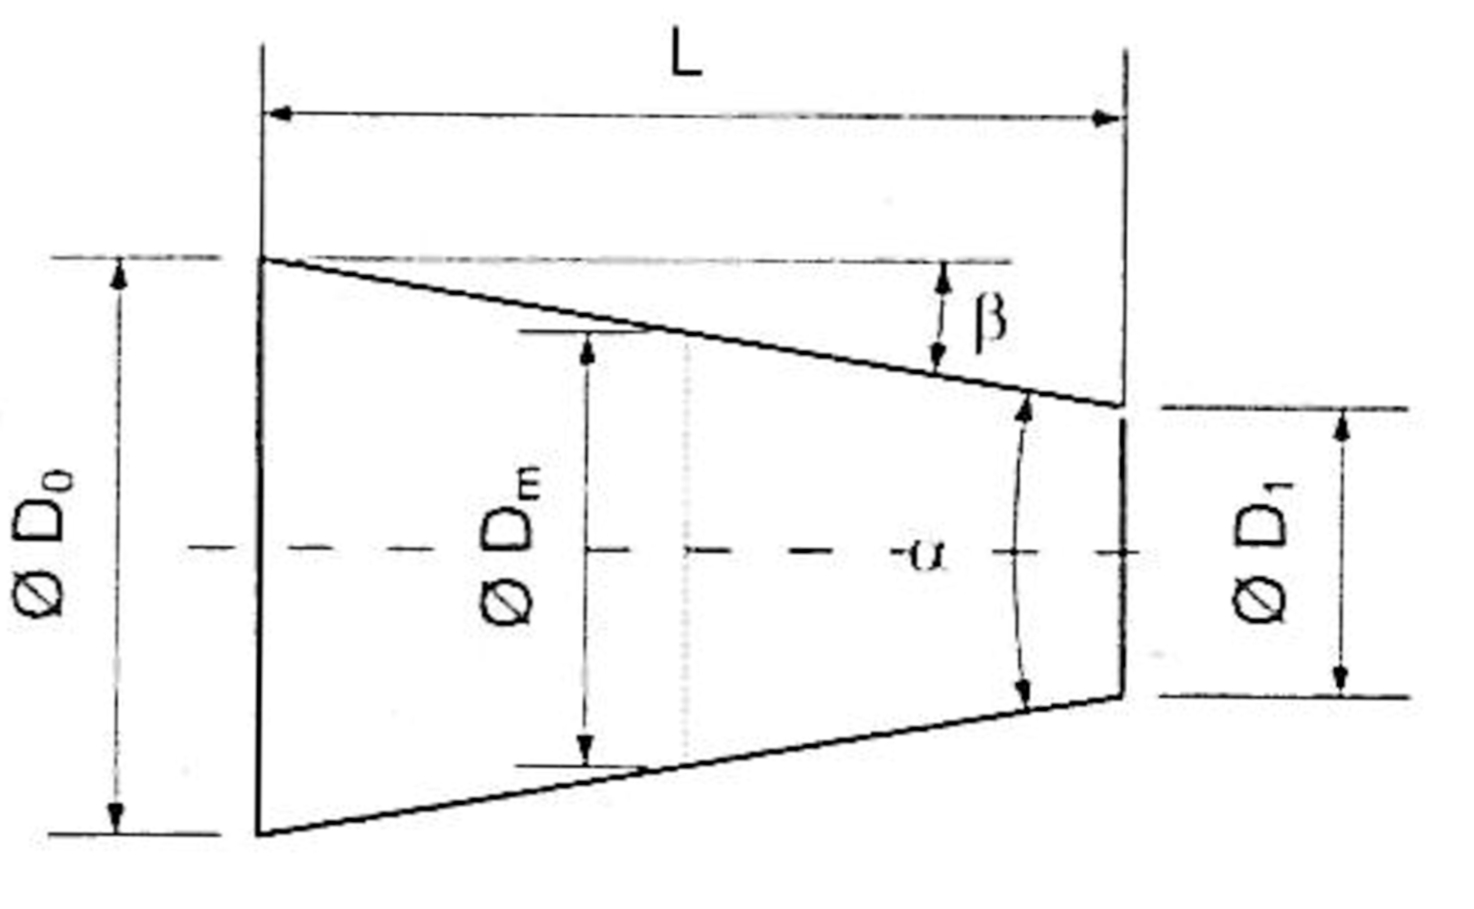
\includegraphics[width=0.6\linewidth]{kupplungen/kegel-welle}
		\caption*{Geometrie des Kegels}
		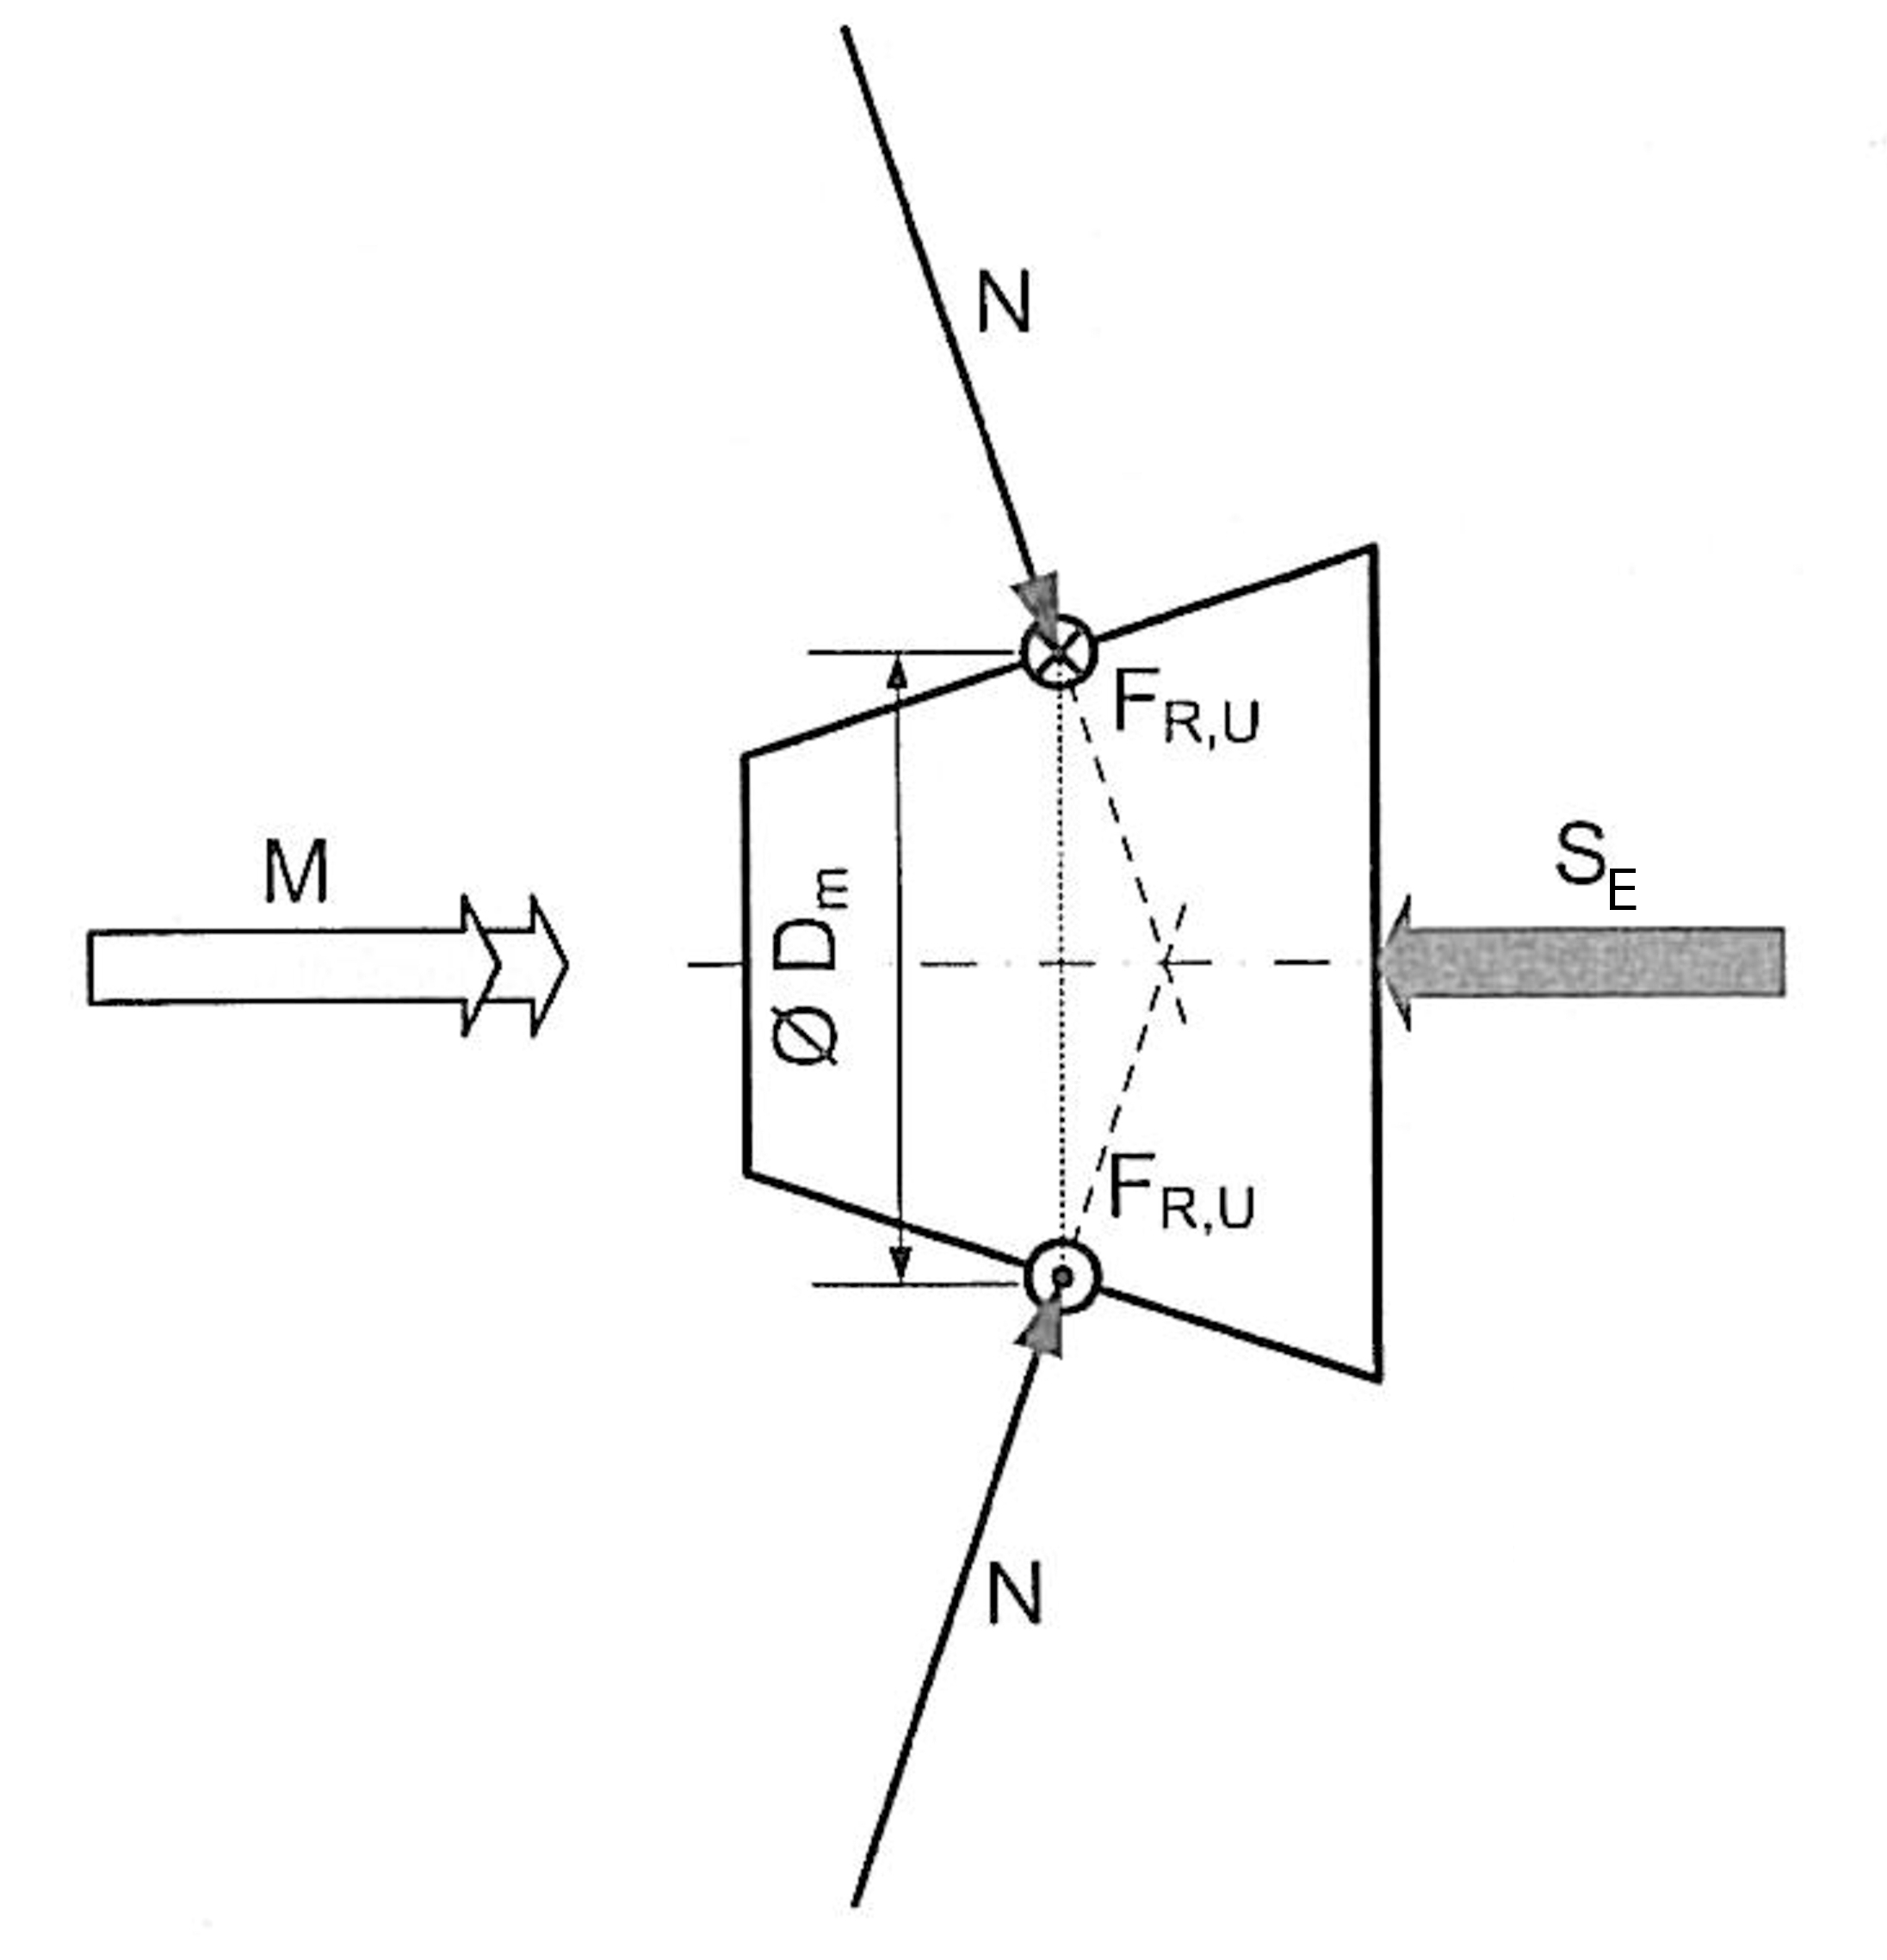
\includegraphics[width=0.6\linewidth]{kupplungen/kegel-welle-frei}
		\caption*{Krafteinwirkung auf den Kegel}
\end{figure}

% Mittlerer Durchmesser
\begin{eeqn}{Mittlerer Durchmesser}
	\begin{align}
		D_\text{m} &= \frac{D_0+D_1}{2}
	\end{align}

\end{eeqn}

% Kegelverhältnis
\begin{eeqn}{Kegelgeometrie}
	Kegelverhältnisse werden als $\rhd\;x:y$ angegeben. Dies entspricht:
	\begin{align}
		C & = \frac{x}{y} = \frac{D_0-D_1}{L}
	\end{align}
	Beispiel: $\rhd\; 1:10 \Rightarrow C=0,1$ \\
	Um den halben Öffnungswinkel $\beta$ zu erhalten nutzt man:
	\begin{align}
		\beta & = \arctan \frac{C}{2}
	\end{align}
\end{eeqn}

% Übertragbares Drehmoment
\begin{eeqn}{Übertragbares Drehmoment}
	\begin{align}
		M &= \frac{S_\text{E} \cdot \mu \cdot D_\text{m}}{2\cdot (\sin \beta + \mu \cdot \cos \beta)}
	\end{align}
	Auslegungsgleichung für Kegel-Welle Verbindungen
\end{eeqn}

% Kegelpressung
\begin{eeqn}{Kegelpressung}
	\begin{align}
		P &= \frac{2\cdot M \cdot \cos \beta}{\mu \cdot \pi \cdot L \cdot D_\text{m}^2}
	\end{align}
	Pressung in der Fuge einer Kegel-Welle Verbindung
\end{eeqn}
\vfill
\pagebreak

\subsection{Klemmverbindungen}
\begin{vardef}
	\item[$D_\text{F}$] Durchmesser der Fuge
	\item[$D_\text{B}$] Bohrungsdurchmesser für die Schraube
	\item[$F_\text{N}$] Gesamte Radiale Spannkraft
	\item[$H$] Höhe der Klemmverbindung
\end{vardef}

% geteilte (biegesteife) Klemmverbindung
\hrule
\begin{eeqn}{geteilte (biegesteife) Klemmverbindung}
	\begin{align}
		M &= \mu \cdot F_\text{N} \cdot D_\text{F}
	\end{align}
	Die Klemmen werden bei diesem Typ auf Spielpassung ausgelegt. Die Krafteinleitung erfolgt über zwei Punkte.
\end{eeqn}

% geteilte (biegeweiche) Klemmverbindung
\begin{eeqn}{geteilte (biegeweiche) Klemmverbindung}
	\begin{align}
		M &= \mu \cdot F_\text{N} \cdot D_\text{F} \cdot \frac{\pi}{2}
	\end{align}
	Die Klemmen werden bei diesem Typ auf Presspassung ausgelegt. Die Krafteinletung erfolgt über die gesamte Mantelfläche der Welle.
\end{eeqn}

\begin{figure}[H]
	\centering
	\begin{minipage}[b]{0.49\linewidth}
		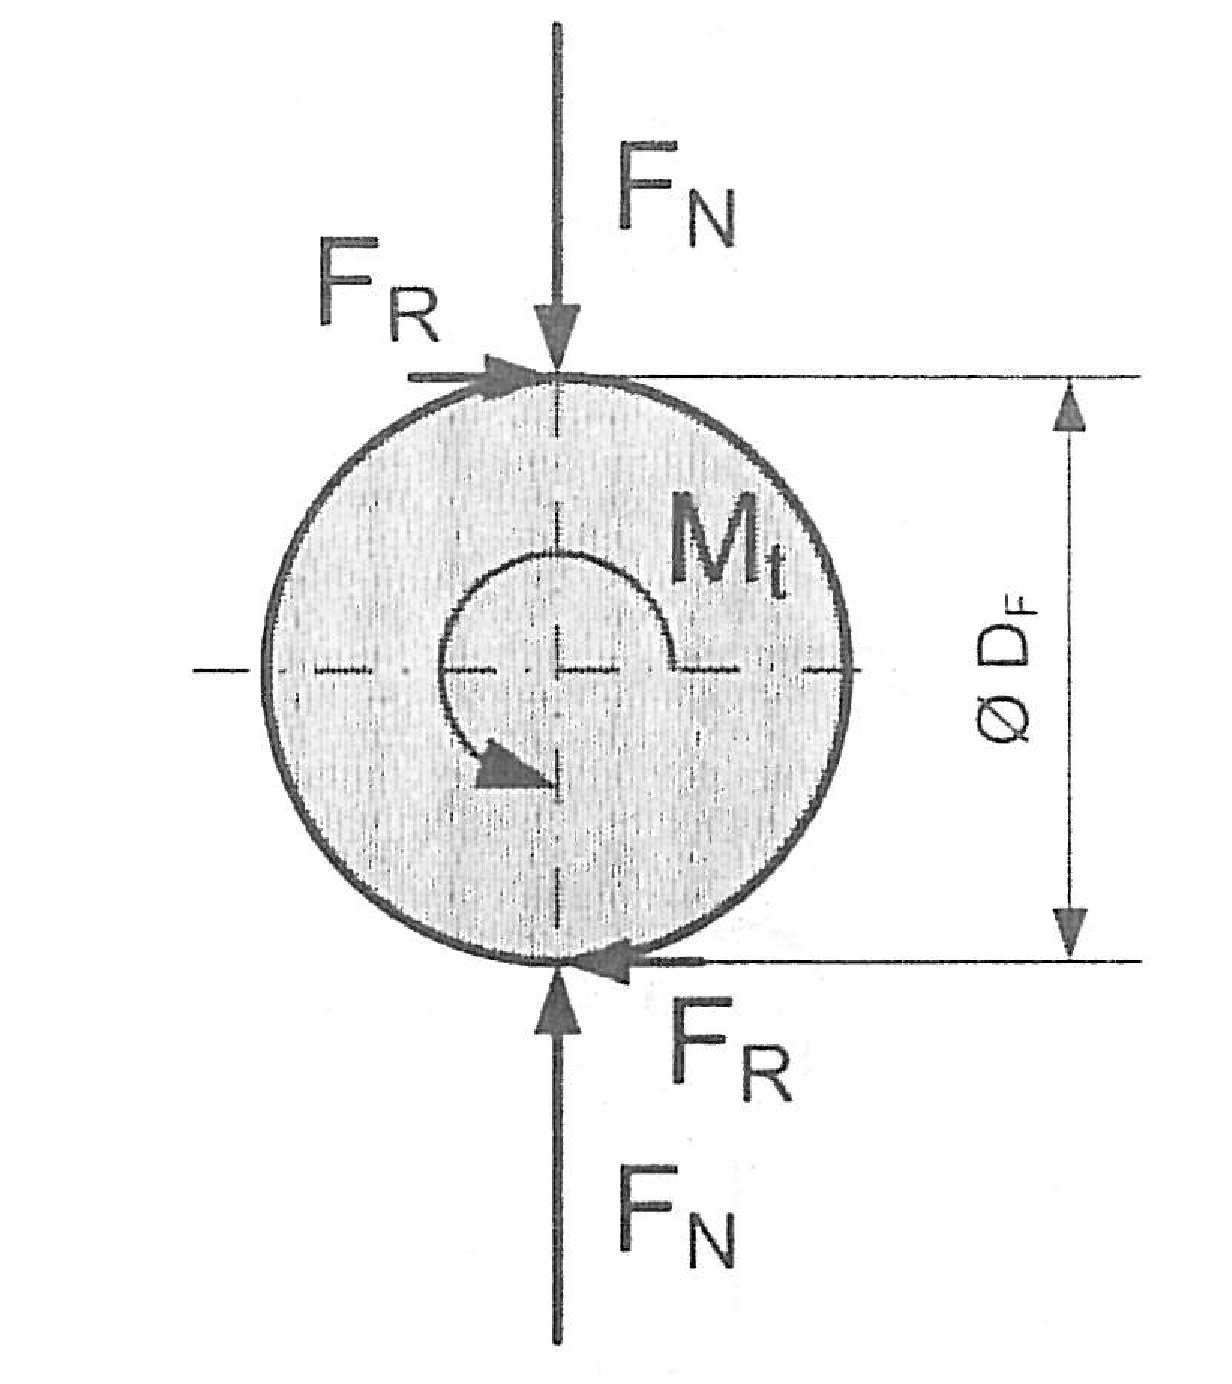
\includegraphics[width=\linewidth]{kupplungen/klemmverbindung-starr}
		\caption*{Biegestarre Klemmverbindung}
	\end{minipage}
		\begin{minipage}[b]{0.49\linewidth}
		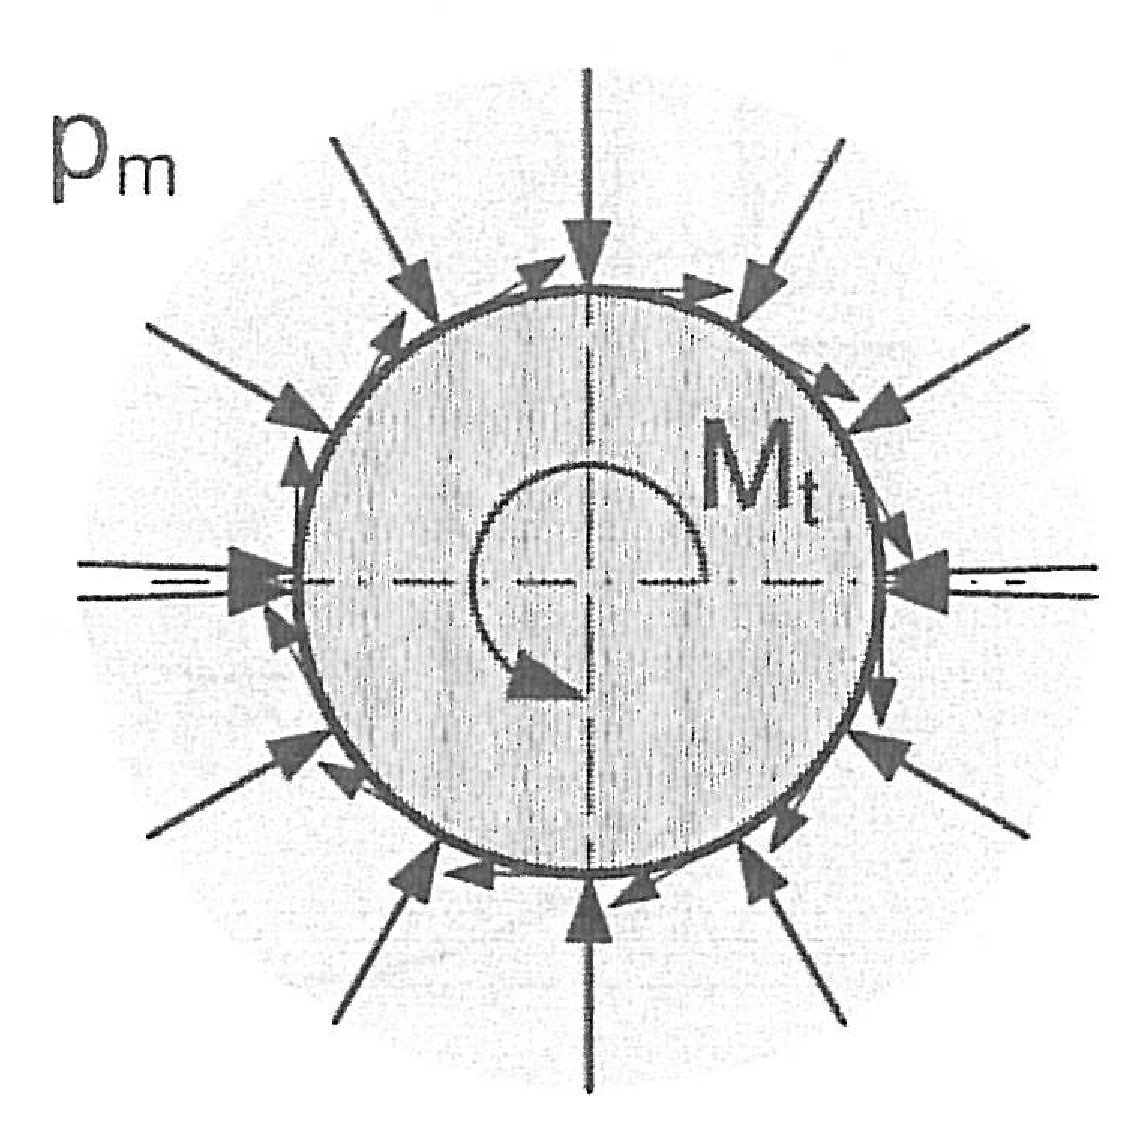
\includegraphics[width=\linewidth]{kupplungen/klemmverbindung-weich}
		\caption*{Biegeweiche Klemmverbindung}
	\end{minipage}
\end{figure}

\pagebreak
% geschlitzte Klemmverbindung
\hrule
\begin{eeqn}{geschlitzte Klemmverbindung}
	\begin{align}
		& M = 2\cdot F_\text{S} \cdot \frac{a+k}{b} \cdot \mu \cdot D_\text{F} \\
		& P = \frac{F_\text{N3}}{l\cdot D_\text{F}}
	\end{align}
	In der Verbindung treten folgende Kräfte auf:
	\begin{align}
		&F_\text{N 1,2} = S \cdot \frac{a+k}{b} \\
		&F_\text{N3} \approx 2 \cdot F_\text{N 1,2}
	\end{align}

	Für die Konstanten $a, b, k$ gelten folgende Näherungen:
	\begin{align}
		&a  \approx 0,5 \cdot D_\text{B} + 0,5 \cdot D_\text{F}+ c\\
		&c \approx 0,1 \cdot D_\text{F}\\
		&b \approx \frac{H+D_\text{F}}{4} \\
		&k \approx 0,1 \cdot D_\text{F} \qquad (k\approx 0,05 \cdot D_\text{F} \ldots  0,2 \cdot D_\text{F})
	\end{align}
\end{eeqn}

\begin{figure}[H]
	\centering
	\begin{minipage}[b]{0.48\linewidth}
		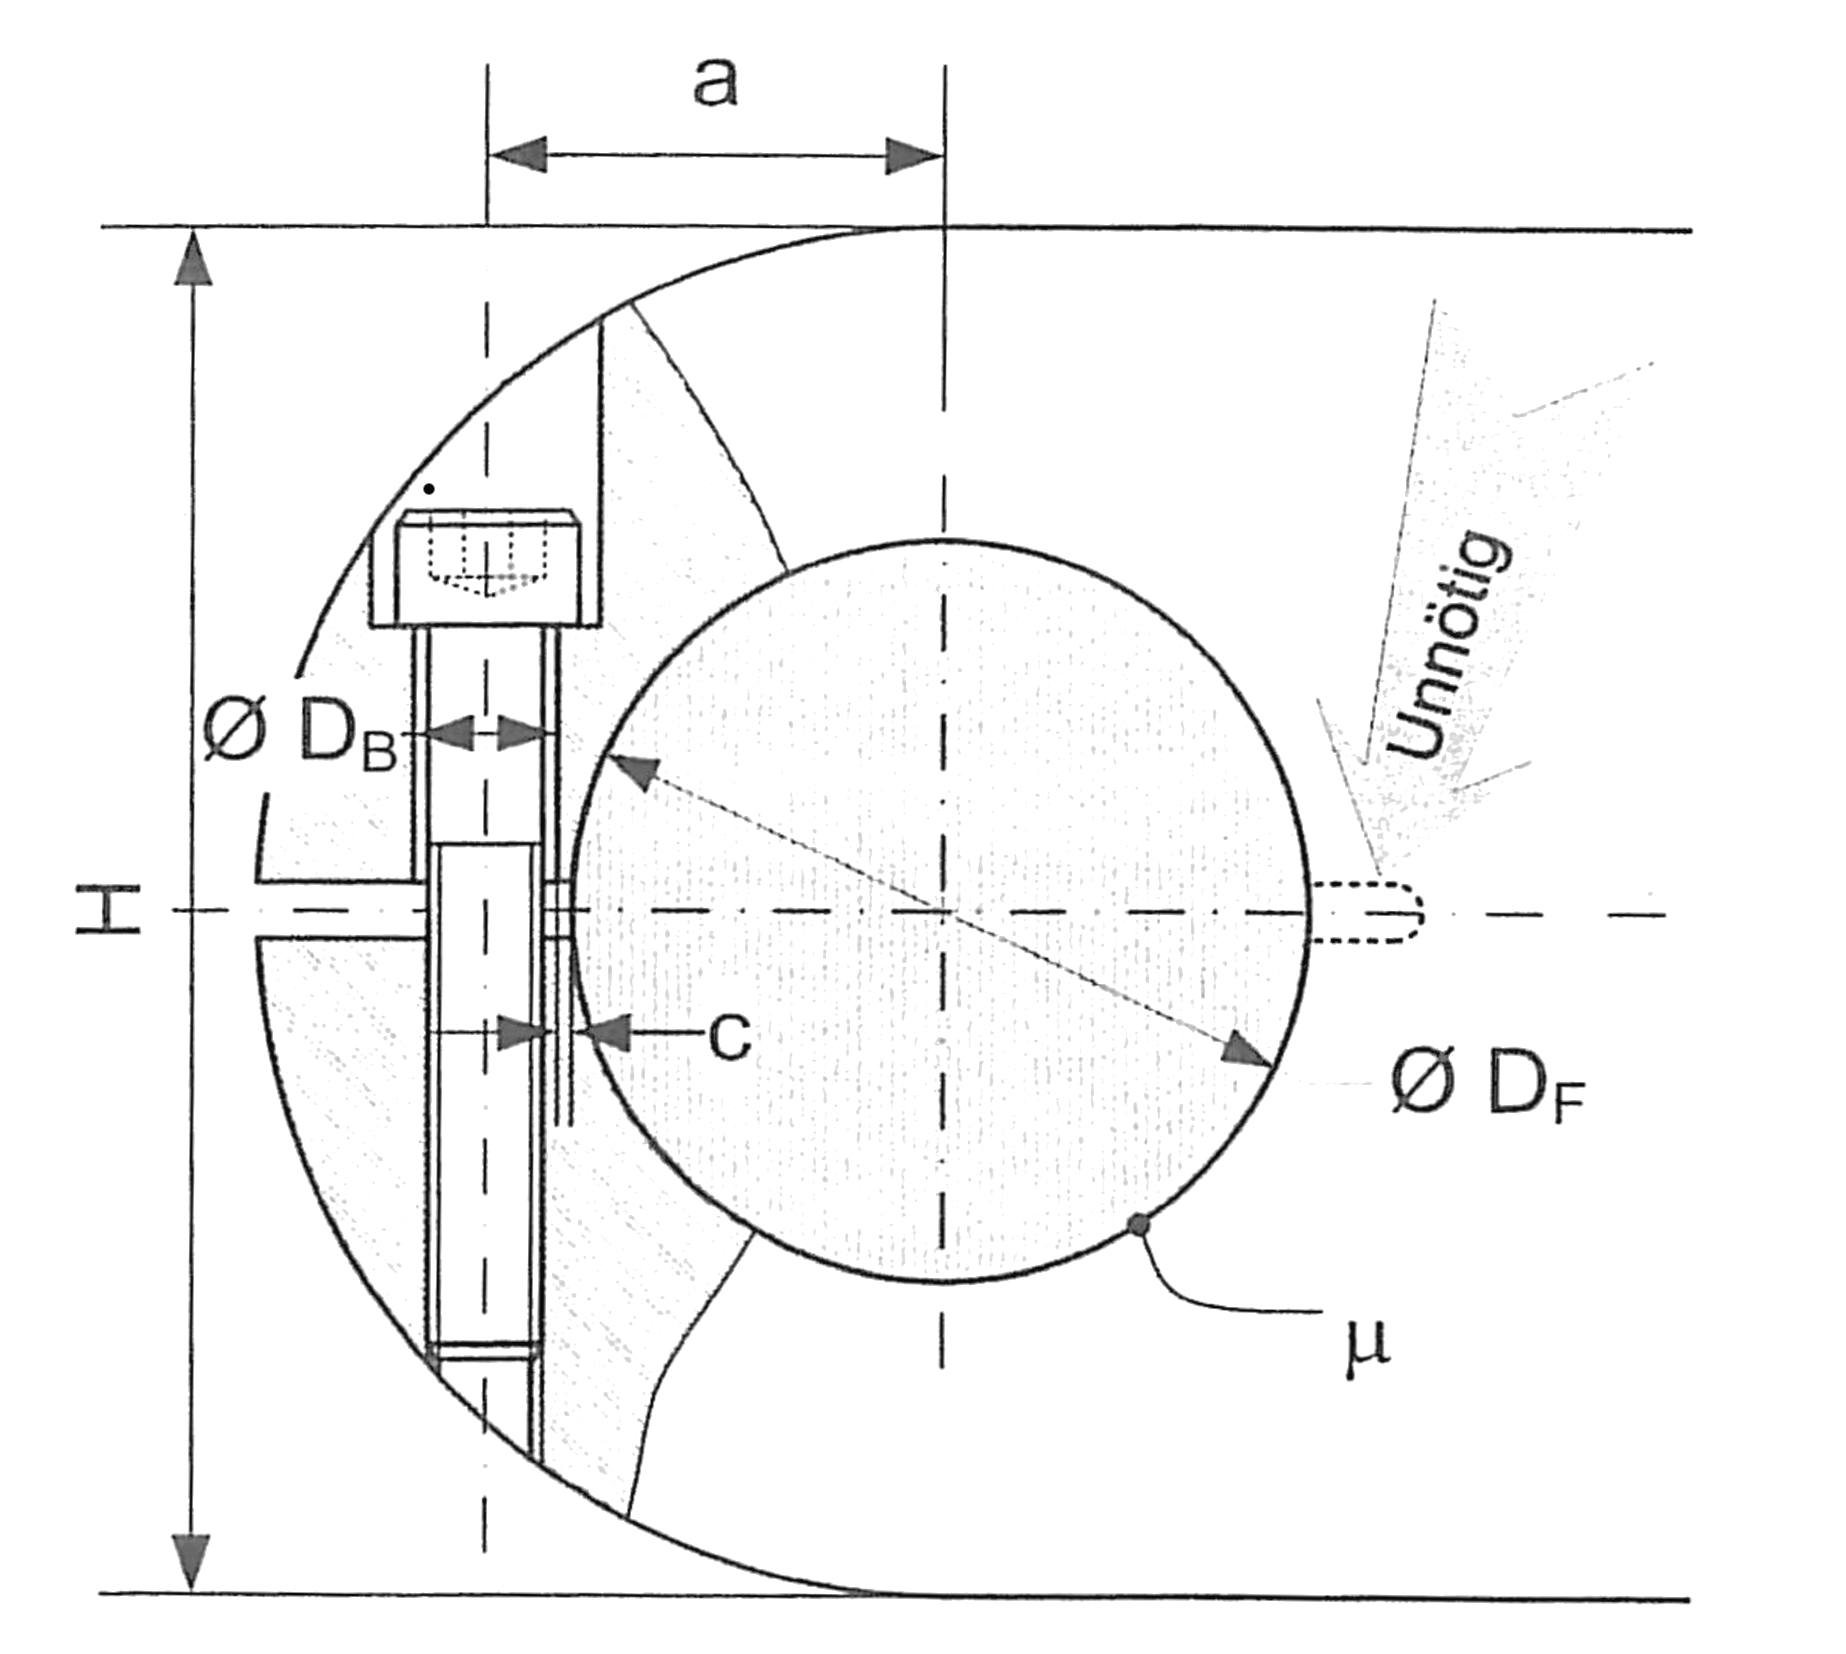
\includegraphics[width=\linewidth]{kupplungen/geschlitzte-klemmverbindung}
		\caption*{Geschlitze Klemmverbindung}
	\end{minipage}
		\begin{minipage}[b]{0.48\linewidth}
		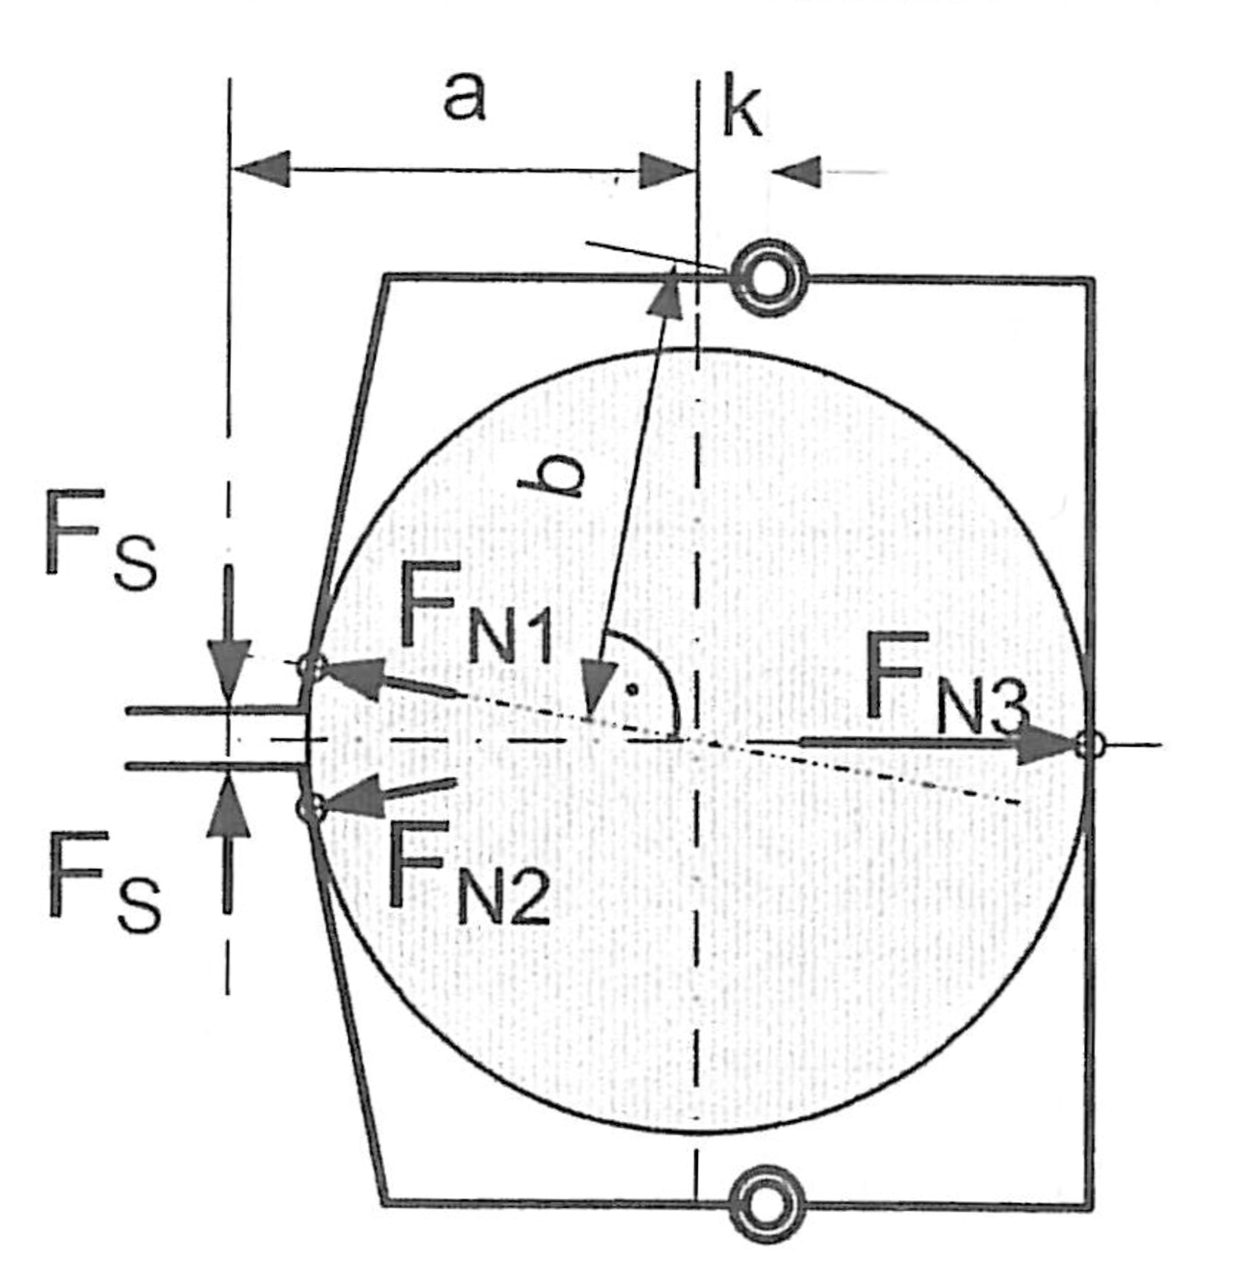
\includegraphics[width=\linewidth]{kupplungen/geschlitzte-klemmverbindung-frei}
		\caption*{Krafteinwirkung}
	\end{minipage}
\end{figure}

	\section{Sonstiges}
\hrule
%Reibung an Kreisringen
\begin{eeqn}{Reibung an Kreisringen}
	\begin{align}
		& M_\text{R} = F_\text{S}\cdot r_\text{m} \cdot \mu \\
		& r_\text{m} = \frac{D_\text{a}+D_\text{i}}{4}
	\end{align}
	Das Reibmoment $M_\text{R}$ entspricht einem Drehmoment, dass ensteht wenn ein Kreisring auf einer Oberfläche gedreht wird. Es wirkt der eigentlichen Drehbewegung entgegen.
\end{eeqn}

% Pressung auf nicht ebene Flächen
\begin{eeqn}{Pressung auf nicht ebene Flächen}
	\begin{align}
		P = \frac{F}{A_\text{proj}}
	\end{align}
\end{eeqn}

% Mehrschnittige Scherspannugen
\begin{eeqn}{mehrschnittige Scherspannugen}
	Wenn ein Element an $n$ Stellen gleichzeitig angeschert wird, spricht man von einer $n$-schnittigen Verbindung:
	\begin{align}
		\tau_\text{A} = \frac{F}{A\cdot n}
	\end{align}
\end{eeqn}

% Seilreibung (Eytelwein'sche Reibung)
\begin{eeqn}{Seilreibung (Eytelwein'sche Reibung)}
	Wenn ein Seil eine Achse mit dem Winkel $\alpha$ umschlingt, gilt für die Reibung:
	\begin{align}
		\frac{S_1}{S_2} = e^{\mu \cdot \alpha}
	\end{align}
\end{eeqn}

% Sicherheitsbeiwert
\begin{eeqn}{Sicherheitsbeiwert}
	\begin{align}
		S &= \frac{F}{F_\text{zul}}
	\end{align}
\end{eeqn}

% Leere Seiten am Ende
\pagestyle{empty}
\clearpage
\section*{ }
\clearpage
\section*{ }
\end{document}
